%% uctest.tex
%% See accompanying LICENSE file for licensing, history, and copyright
%% information.

% This line is required for LPPL compliance.
\message{You are using a modified uctest.tex}
% Note that if you turn this file into a Derived Work that is not intended as a
% replacement for the original template (i.e. an actual thesis), and you do not
% imply that anyone provides support for your modified version, you may
% distribute it under any license you wish.

\documentclass[11pt]{ucscthesis}
\def\dsp{\def\baselinestretch{2.0}\large\normalsize}
\dsp

% 2010june01 sol katzman:
% package geometry should override the various margin settings from .clo and .cls
% and also eliminates issues where the default papersize is A4
\usepackage[letterpaper, left=1.5in, right=1.25in, top=1.25in, bottom=1.25in, includefoot]{geometry}
% Use PostScript fonts as required by UCSC Dissertation Preparation Guidelines
\usepackage{pslatex}
\usepackage{url}
\usepackage{graphicx,epsfig}
\usepackage{blindtext}
\usepackage{natbib}
\usepackage{amsmath}
\usepackage{tabularx}
%Fixing a problem with the ucthesis.cls compatibility with the natbib package 
\def\newblock{\hskip .11em plus.33em minus.07em}
\newcommand{\onepic}{.4}
\newcommand{\Fermi}{{\it Fermi }}
\newcommand{\FermiLAT}{{\it Fermi}-LAT }
\begin{document}

% Declarations for Front Matter

\title{Searching for New Physics with {\it{Fermi}}-LAT}
\author{Arne C. Johnson III}
\degreeyear{2018}
\degreemonth{August}
\degree{DOCTOR OF PHILOSOPHY}
\chair{Professor Ignatius Arrogant}
\committeememberone{Professor Ivory Insular}
\committeemembertwo{Professor General Reference}
\committeememberthree{Professor Ipsum Lorem}
\numberofmembers{4} %% (including chair) possible: 3, 4, 5, 6
\deanlineone{Dean John Doe}
\deanlinetwo{Vice Provost and Dean of Graduate Studies}
\deanlinethree{}
\field{Physics}
\campus{Santa Cruz}

\begin{frontmatter}

\maketitle
\copyrightpage

\tableofcontents
\listoffigures
\listoftables

\begin{abstract}
Theses have elements.  Isn't that nice?

\end{abstract}

\begin{dedication}
\null\vfil
{\large
\begin{center}
To myself,\\\vspace{12pt}
Perry H. Disdainful,\\\vspace{12pt}
the only person worthy of my company.
\end{center}}
\vfil\null
\end{dedication}


\begin{acknowledgements}
I want to ``thank'' my committee, without whose ridiculous demands, I
would have graduated so, so, very much faster.
\end{acknowledgements}

\end{frontmatter}

%\part{Introduction}
\chapter{Introduction}
The Standard Model of particle physic has enjoyed an unprecedented level of success since its completion in the late 1960s. Together with Einstein's theory of general relativity, today's physicists possess the ability to understand Nature on both the smallest and largest of scales.
The legacy of the Standard Model has been bolstered in recent years by several experimental achievements. The discovery of the Higgs boson by the ATLAS \cite{the_atlas_collaboration_observation_2012} and CMS \cite{the_cms_collaboration_observation_2012} teams at the Large Hadron Collider in the summer of 2012 completed the Standard Model's last missing link. Further analyses by ATLAS and CMS have since confirmed that the discovered Higgs boson has exactly the predicted properties and couplings to other particles. The discovery of gravitational waves in 2015 by the LIGO experiment \cite{ligo_scientific_collaboration_and_virgo_collaboration_observation_2016} provided spectacular confirmation of one of the most intriguing predictions of general relativity. Our understanding of the Universe has never been on such sure footing.
And yet for all its successes, the Standard Model remains at best frustratingly incomplete. Astronomical observations indicate the presence of large amounts of dark matter, whose mass dwarfs that of the Standard Model components. And although no experiment to date has seen significant deviations from the predictions of general relativity or the Standard Model, the two theories are known to be incompatible on a fundamental level. With careful experimentation, physicists can study these problems head-on, and perhaps make progress towards addressing them. 

\section{Dark Matter}
Multiple lines of inquiry have firmly established that a majority of the mass-energy density of the Universe is composed of a component which is neither baryonic nor luminous. The first indications of what we now call dark matter (DM) were Zwicky's observations in 1933 that the velocity dispersion of galaxies in the Coma Cluster was far higher than the escape velocity predicted from the mass of the luminous galaxies \cite{zwicky_1933}. Later observations of galaxy clustering, for example Kahn \& Woltjer's analysis of the motion of Andromeda \cite{kahn_intergalactic_1959}, further indicated that galaxies were far more massive than conventionally expected. The evidence continued to mount in the 1970s as work done by Rubin \& Ford \cite{rubin_rotation_1970} and Roberts \& Rots \cite{roberts_comparison_1973} showed that the rotation curve of Andromeda was flat out to large distances (30 kpc) from the galactic center, indicating that the mass-to-light ratio at large radii was far larger than that of a typical star. Further data from Rubin \cite{rubin_extended_1978} subsequently confirmed that the same result held true for a nearly all spiral galaxies she considered. 
 
The mystery deepened as it became clear that the dark matter could not be composed of traditional baryonic matter. The most visceral indication of this fact comes from a comparison of the gravitational lensing by merging galaxies in the Bullet Cluster to an X-ray tracer of the gas content \cite{clowe_direct_2006}. The data shows conclusively that although the gas dominates the visible mass of the cluster, the lion's share of the mass undergoes little self-interaction. Moreover, Big Bang nucleosynthesis (BBN) constrains the baryonic density of the the Universe to be less than about one twentieth of the critical density, but the astronomical observations indicate that the DM density is approximately a quarter of the critical density. The scale of temperature fluctuations in the CMB is also too small to account for the observed density clustering in today's Universe, but the problem can be resolved if the Universe has a large nonbaryonic component \cite{einasto_dark_2009}.

Today, DM plays a key role in the successful $\Lambda$CDM model of the Universe by seeding density fluctuations around which galaxies grow.
N-body simulations of galaxy formation with cold dark matter have shown great success at reproducing the observed structure \cite{bertone_particle_2010}.
The exact nature of the DM, however, remains unkown.
The known massive neutral particles in the Standard Model (e.g. the Higgs or Z bosons, the neutron) all decay too quickly to account for the presence of DM at the current time. Of the remaining neutral particles, the only plausible candidates are the neutrinos, but their low mass precludes them from moving slowly enough to form structures as small as galaxies \cite{einasto_dark_2009}. 

A variety of candidates for the identity of dark matter have been proposed, most of which require extensions to the Standard Model. 
These extensions invariably predict the existence of new neutral, stable particles, of which the most widely studied are axions and WIMPs.

\subsection{Axions}
The motivation for axions comes from the strong CP problem- the question of why CP symmetry is conserved to a high degree in the strong interaction despite the O(1) CP-violating phase in the weak interaction. Assuming the Universe is not fine-tuned, CP violation in QCD can be made small dynamically by the introduction of a new U(1) symmetry (the Peccei-Quinn symmetry). The Nambu-Goldstone bosons of this new symmetry are the axions, in much the same way as the photon is the Goldstone boson of the U(1) symmetry associated with the electromagnetic interaction. 
If they exist, axions must have extremely small masses and low couplings to Standard Model particles. Constraints from beam-dump experiments and astrophysical searches require the axion mass to be less than approximately $10^{-3}$ eV. On the other hand, the axion mass must be greater than approximately $10^{-6}$ eV in order to not overclose the Universe \cite{bertone_particle_2010}. If the axion mass is near its lower bound, axions are a plausible DM candidate. Although lighter than neutrinos, the density fluctuations in the axion field are localized enough to reproduce the DM substructure that we observe. A variety of experiments to search for them are underway, which generally seek to excite the axion field and produce resonant photons via the Primakoff process. 

\subsection{WIMPs}
Weakly Interacting Massive Particles (WIMPs) are a class of particle which generally possess masses and coupling strengths on the order of the electroweak scale (roughly 100 GeV). 
Such particles would have been in thermal equilibrium with the rest of the matter at moments shortly after the Big Bang, but as the Universe expanded and cooled, the WIMPs would have ceased to be in equilibrium when the Hubble rate exceeded the interaction rate. As it turns out, a weak-scale cross-section yields dark matter that "freezes out" from the rest of the Universe at precisely the correct time to yield the observed relic abundance, a coincidence which has been dubbed the 'WIMP miracle' \cite{bertone_particle_2010}.

Generally speaking, there are three paradigms through which to search for WIMP dark matter.
WIMPs can be produced in collisions at high-energy particle accelerators like the LHC. In this case, the stable and neutral WIMPs will escape the detector apparatus, leading to "missing" transverse momentum in the reconstructed final state of particles. The scattering of WIMPs off of nucleons can also be searched for by low-background counting experiments. These experiments are typically performed deep underground to avoid contamination by showers from cosmic rays.
Finally, WIMPs may annihilate or decay to Standard Model particles, which we can detect by looking at areas in the Universe where we know high concentrations of dark matter exists. WIMP annihilation in the context of such 'indirect detection' experiments will be the focus of Sections X \& Y. 

\subsection{PBHs}
Unlike many other dark matter candidates, primordial black holes (PBHs) are attractive as dark matter candidates because they require little in the way of new physics beyond the Standard Model (theories of the early Universe notwithstanding). They also present straightforward detection strategies- heavy PBHs can in principle be detected via the gravitational wave events from their mergers; intermediate-mass PBHs can be constrained by their accretion onto neutron stars and white dwarfs \cite{pani_tidal_2014} or potentially detected via microlensing events \cite{carr_primordial_2016}. Low-mass PBHs can be detected by their Hawking radiation; a more detailed discussion of PBHs as dark matter candidates and the prospects for detecting low-mass PBHs will follow in Section X. 

\section{Quantum Field Theory in Curved Spacetime}
Although general relativity and the Standard Model excel at describing Nature on large and small scales, respectively, a complete theory of quantum gravity remains unknown. Theorists have had some success (see the results in Section X, for instance) in describing quantum field theories in a background of curved spacetime, but generally these models neglect perturbative interactions in favor of free fields. 
As noted in Wald \cite{wald_general_1984}, the source of the difficulty in constructing a completely satisfactory theory of quantum gravity is rooted in the fact that the metric $g_{\mu\nu}$ is both the dynamical variable of general relativity and the description of the spacetime in which the quantum theory lives.
Attempts to construct perturbative theories of gravitation via Einstein's equation for a massless spin-2 field have failed due to the fact that these theories are generally nonrenormalizable.

In the face of these theoretical challenges, unfortunately, experiments also offer little guidance.
The problem for experimentalists is essentially one of mismatched scales: gravitation is extraordinarily weak on the scale of a typical quantum system (a rough sense of the mismatch is given by the fact that Newton's gravitational constant is some 42 orders of magnitude weaker than the Coulomb constant).
The Planck scale (roughly $10^{18}$ GeV), where GR effects become important, is far beyond the reach of even the most ambitious particle accelerator designs.
Only a handful of instances exist where general relativity can conceivably be applied to a quantum system- the Big Bang, for instance.
Observing the Big Bang directly in the electromagnetic spectrum is made difficult by the presence of the cosmic microwave background (CMB).
Future experiments, however, may be able to detect primordial gravitational waves (either directly or via B-mode polarizations in the CMB) that are predicted to arise from models of inflation and thus provide a crucial test of theories of the Big Bang.
Alternatively, PBHs provide a natural laboratory for observing physics at the Planck scale: as PBHs evaporate, their temperature diverges towards the Planck scale and necessarily new physics will describe their dynamics. A search for PBHs in this context is described in Sections X \&Y.

In the work that follows I present two analyses that make use of data from the Fermi Large Area Telescope (Fermi-LAT) to search for evidence of dark matter and PBHs. I will show that the capabilities of {\it{Fermi}}-LAT allow it to test models of physics that cannot be studied with other means. Gamma-ray astrophysics remains one of the best available probes of physics beyond the Standard Model.


\chapter[\FermiLAT and the $\gamma$-Ray Sky]{\FermiLAT and the $\gamma$-Ray Sky}
In this chapter I provide an overview of the design and analysis abilities of the Large Area Telescope on board the \Fermi Gamma Ray Space Telescope (otherwise known as \FermiLAT). \FermiLAT is a whole-sky imaging gamma-ray telescope currently in low-Earth orbit which is capable of detecting photons from about 10 MeV to more than 1 TeV in energy. For a more in-depth description of the LAT design, the \FermiLAT collaboration provides technical paper \cite{collaboration_large_2009}. 

\section{History}
The field of gamma ray astronomy begins in earnest with a paper by Morrison in 1958 \cite{morrison_gamma-ray_1958} which lays out the motivation for making astronomical observations at high energies. The crux of Morrison's argument is that visible light from high-energy processes is only created indirectly- the nuclear reactions that power stars, for example, are screened by huge amounts of stellar medium. High-energy charged particles are directly produced by energetic processes, but they are deflected by magnetic fields, obscuring their origin. Gamma rays, on the other hand, are produced directly in high-energy processes and are unaffected by magnetic fields, therefore providing a window into new physical processes. 

Morrison's ideas were influential in the creation of a number of balloon-based gamma ray instruments, as well as the space-based telescopes {\textit {Agile}} and EGRET. A proposal for the telescope that would eventually become \Fermi-LAT was first put together in 1994. During the next 14 years, an international collaboration of scientists and engineers, primarily from the United States, Italy, Japan, and Sweden worked together to build \Fermi. On June 11, 2008, the \Fermi Gamma Ray Space Telescope was successfully launched into low-Earth orbit aboard a Delta II Heavy launch vehicle. In its ten years in orbit, \Fermi has successfully measured the angular positions, energies, and arrival times of over 1 billion photons. 

\section{Design}
The design of \FermiLAT is informed by the fact that gamma rays cannot be focused or reflected in the same manner as visible light, as their wavelength is far smaller than typical atomic spacing. Instead of measuring the gamma rays directly, \FermiLAT causes incident gamma rays to pair-convert into electrons and positrons whose momenta are then measured. Pair-conversion is an important background rejection feature, as only e+/e- pairs that originate from within the LAT are eligible gamma-ray candidates. The measurement of the e+/e- momenta takes place in two stages- directional information is reconstructed from hits in silicon strip sensors in the tracker, while energies are measured via detection of scintillation light in the calorimeter.

\subsection{Tracker}
There are 16 individual tracker towers on the LAT, arranged in a 4x4 grid. Each tower has 18 double layers of orthogonally-oriented silicon strip detectors. 16 layers of a high-Z material (tungsten foil) are placed in front of each of the first 16 pairs of silicon strip detectors, providing a location where the gamma rays can pair-convert into an electron and positron. Electron/hole pairs are created in the silicon detectors as the pair-produced electrons and positrons pass through them, which are then read out by electronics. The recorded positions of the electron/positron pair are recorded at each subsequent tracker layer, and a track reconstruction algorithm (generally based on a Kalman filter) is used to find the path of the e+ and e-.

As the e+/e- pairs traverse the tracker layers, they undergo multiple scattering (especially by the tungsten foils), which limits the angular resolution available. On the other hand, the probability of a gamma ray conversion event is proportional to the thickness of the tungsten, so a compromise between two competing goals (good angular resolution and high conversion efficiency) must be reached. In the LAT, the compromise made was to separate the tungsten into two groups: the first 12 layers are relatively thin (the "front") while the last 4 layers ("back") are approximately 6 times thicker. The total number of radiation lengths is approximately equal in the "front" and "back" segments, though the front-converting photons have somewhat better angular resolution, by roughly a factor of two.
The angular resolution of \FermiLAT for "front"- and "back"- converting photons is represented in Figure X by the 68\% containment radius. Notably, the resolution improves dramatically as the energy of the incident photon increases- this is a consequence of the fact that a typical multiple scattering angle is inversely proportional to the energy of a particle.

\subsection{Calorimeter}
Below each tracker tower lies a calorimeter module containing 96 scintillating thallium-doped cesium iodide crystals, read out by PIN photodiodes. The crystals are oriented in 8 rows of 12 crystals in a hodoscopic array, yielding a total calorimeter depth of 8.6 radiation lengths. As the primary high-energy electrons and positrons from the tracker encounter the dense calorimeter medium, they radiate secondary photons which can themselves pair-produce electron-positron pairs. The process continues until the energy of the gamma rays in the resulting electromagnetic shower falls below the rest energy of an electron, yielding a shower shape that is sensitive to the total energy of the primary electron or positron. 
With its segmented array, the LAT calorimeter modules are capable of measuring both the energy and shape of the electromagnetic shower. The reconstructed energy is simply the sum of all the collected energy in the scintillators, subject to corrections (estimated from Monte Carlo studies) for showers that are large enough to escape the detector volume. The eigenvectors of the shower shape are then computed and used to guess a preliminary track direction to seed the track reconstruction algorithm.

\subsection{Anticoincidence Detector}
Surrounding the tracker and calorimeter is a segmented anti-coincidence detector composed of scintillating plastic, whose purpose is the rejection of charged particle backgrounds from cosmic rays. The material of the ACD is chosen to be low-Z so as to not absorb any gamma-rays, and to not provide a location for incident protons to generate pions (which would generate a substantial background by subsequent decay to two gamma rays). 
Events are vetoed only if the ACD triggers at a position consistent with reconstructed track, which prevents spurious vetos from 'backsplash'- an effect that occurs when the EM shower in the calorimeter causes the emission of secondary particles that strike the ACD. By segmenting the ACD into 89 tiles, these self-veto events are present for less than 20\% of the photons at 300 GeV, compared to ~50\% at 10 GeV for the non-segmented EGRET.

\subsection{Data}
\Fermi most often operates in 'survey mode', during which it scans the entire sky with roughly equal exposure on a time scale of ~3 hours. However, alternate observing patterns are relatively common, such as when \Fermi reorients itself to observe the potential afterglow of a LIGO event, or points towards a flaring blazar for an extened period. Other interruptions to regular data collection include the times \Fermi traverses the South Atlantic Anomaly (during which the event rate becomes extremely high), and the handful of orbits during which \Fermi has faced the Earth in order to detect terrestrial gamma-ray flashes from lightning.

Data collected by \FermiLAT is downloaded via radio link in ~1.5 Gb intervals approximately every 3 hours to NASA's Goddard Space Flight Center, and sent on to SLAC National Accelerator Laboratory for processing to reconstruct photon properties and reject background signals. Photons detected by \FermiLAT are typically available for download from the GSFC within 8 hours of their arrival.

\section{$\gamma$-Ray Sky}
A typical \FermiLAT gamma ray has an energy in the GeV range. An approximate measure for the corresponding temperature of such a photon is given by E/k= $10^13$ K, for comparison, the temperature at the center of the Sun is approximately $10^7$ K. Therefore high-energy gamma rays are generally produced by a handful of non-thermal processes. Relativistic charged particles can emit synchrotron radiation in the presence of magnetic fields, and bremsstrahlung radiation upon interactions with matter. Neutral pions decay to two gamma rays, and excited nuclei can de-excite via the emission of a gamma ray. In Chapter 6, I will discuss the potential for dark matter to annihilate to final states that include gamma rays.
With this in mind, it is not surprising that the gamma-ray sky looks rather different from the sky in the optical band- see Figure X. A number of features are readily apparent from the whole-sky image:
\subsection{Diffuse emission}
Much of the sky's gamma ray emission is in the Galactic plane, and is due to highly energetic charged particles interacting with the interstellar medium. These interaction generally produce neutral pions which then decay to two gamma rays, the energy of which depends on the energy of the initial cosmic ray. 
The origin of high-energy cosmic rays was a mystery for some time, as 2nd-order \Fermi acceleration seemed insufficient to produce particles with energy >10 GeV. A number of authors in the 1970s, however, discovered that collisionless shock boundary of supernova remnants could sufficiently energize charged particles. At the shock boundary, the magnetic field is nearly discontinuous, and 1st order \Fermi acceleration is sufficient to produce charged particles in the many-GeV energy range.
Models of the galactic diffuse emission are generated by the \FermiLAT collaboration by fitting templates of interstellar emission at several wavelengths to observed regions of the $\gamma$-ray sky \cite{acero_development_2016}.
 
Some diffuse emission extends beyond the Galactic plane, and appears to be isotropic across the sky. Most of this isotropic component is believed to originate from unresolved point sources (see below), though some backgrounds of cosmic rays and improperly reconstructed photons from the Earth limb also contribute.
\subsection{Point Sources}

\subsubsection{Blazars}
Most large galaxies contain a rapidly rotating supermassive black hole at their center, some of which actively accrete material. These so-called "active galaxies" possess two main features- a thermal accretion disk, and a relativistic jet aligned along the black hole's rotation axis. When the Earth lies in the direction of a jet axis, the active galaxy is called a blazar and is a bright sources of gamma rays.

The highly relativistic particles in the jet are believed to derive their power directly from the supermassive black hole. Via the Blandford-Znajek process \cite{blandford_znajek_1977}, magnetic fields from the accretion disk which reach inside the black hole's ergosphere can extract rotational energy from the black hole, and the subsequent rotation of the magnetic field causes charged particles to be accelerated to high speeds along the jets. These relativistic particles can then emit gamma rays via synchrotron radiation, bremsstrahlung, or inverse Compton scattering. 
\subsubsection{Pulsars}
Rapidly rotating neutron stars known as pulsars are one of the most numerous point sources in the gamma-ray sky. Surrounded by extraordinarily powerful and rapidly rotating magnetic fields, pulsars emit gamma rays as electrons stripped from their surface emit synchrotron radiation. A small number of pulsars have periods smaller than 1 second, and are referred to as millisecond pulsars; a novel and unresolved population of millisecond pulsars may exist near the Galactic center and contribute to the $\gamma$-ray excess that has been observed there by a number of authors (e.g. \cite{bhakta_searching_2017}).
\subsubsection{Galactic Center}
	The brightest source in the gamma-ray sky by far is the Galactic center, containing the supermassive black hole at the center of the Milky Way located at Sag A*. A number of models have been proposed to explain the gamma-ray emission at Sag A*, generally involving charged particles interacting with the surrounding medium \cite{van_eldik_gamma_2015}. These particles may be injected into the region by tidal disruption of stars by Sag A*. As discussed in Chapter 6, some DM models predict annihilation to occur in the region surrounding Sag A* as well, which may lead to gamma-ray emission.

\section{Analysis Tools}

\FermiLAT data and LAT-specific analysis tools are publicly available for download from the \Fermi Science Support Center at NASA's Goddard Space Flight Center \footnote{{\tt https://fermi.gsfc.nasa.gov/ssc/}}. 
Processing \FermiLAT data for analysis begins by removing photons (via the tool {\tt gtselect}) that are incident from near the Earth limb, as these mostly originate from cosmic ray interactions with the atmosphere. For a typical analysis, the photons are then binned (with the use of the tool {\tt gtbin}) in angular position and energy. The LAT effective area is convolved (by use of the tool {\tt gtltcube}) with its pointing history over the time period considered to produce an exposure map binned in energy and angular position. 
Typical \FermiLAT analyses make use of maximum likelihood techniques to test differing hypotheses (spectral features, location, etc) about sources in question. The process begins by defining a model of the region of interest (ROI). A model is composed of a list of sources, each of which is defined by its spectral shape, position on the sky, and spatial appearance. With a model and the exposure map, the expected number of photons $\mu_i$ in each bin $i$ can be computed and compared to the actual counts $n_i$. The value of the likelihood for the model is then given by the product of Poisson factors over the number of bins $N$:
\begin{equation}
\mathcal{L} = \prod_{i=1}^{N} \frac{\mu_i^{n_i}}{n_i!}e^{-\mu_i}
\end{equation}
By varying the parameters in the model, the likelihood can be maximized. In cases with sufficient statistics and where the parameters satisfy Wilks criteria, the value of the delta log-likelihood between two hypotheses follows a $\chi^2$ distribution \cite{wilks_1938}. If this is the case, the significance of the varied parameter can be determined; if this is not the case, the significance can be determined through a Monte Carlo study.

The \FermiLAT collaboration has successfully used these techniques to compile several catalogs of gamma-ray sources. The most current catalog is the Third \Fermi Source Catalog \cite{collaboration_fermi_2015} (hereafter referred to as 3FGL). The 3FGL composed of 3033 sources, of which a majority (3008) of which are point sources and 25 of which are modeled as extended. A large fraction of the sources are pulsars or active galaxies, but a sizable component (1010) are unassociated with any known sources. I make use of the 3FGL in Chapter 4 to identify potential PBH candidates, and to place limits on their presence.
\chapter[Black Holes]{Black Holes}
This chapter provides background information on black holes

\section{History}

\section{Theory}
Einstein's equation (in natural units, i.e. $c, h = 1$) is:
\begin{equation}
G_{\mu\nu} = 8\pi T_{\mu\nu}
\end{equation}
The unique static, spherically-symmetric solution to Einstein's equation is the Schwarszchild metric
Schwarszchild metric
\subsection{Hawking Radiation}
In the classical treatment, black holes have no temperature and do not emit blackbody radiation; intuitively, energy cannot escape a black hole because the worldlines of particles inside the event horizon cannot exceed $r=2GM$. 
Interestingly, however, black holes have been shown to exhibit many of the same properties as classical thermodynamic systems.
During black hole mergers, for instance, the total black hole surface area is nondecreasing.
One can draw analogy between properties of black holes and thermodynamic quantities like so:
\begin{tabular}{ccc}


Temperature & $\longleftrightarrow$ & Surface Gravity $\kappa$\\
Entropy & $\longleftrightarrow$ & Surface Area\\
Energy & $\longleftrightarrow$  & Mass\\

\end{tabular}

However, the work of Hawking and Beckenstein in the 1970s led to the understanding that black holes are really cool.
The Hawking temperature of a black hole is given by:
\begin{equation}
T = \frac{\hbar c^3}{8\pi k_B GM}
\end{equation}

As the black hole emits radiation, it loses mass and becomes hotter.
This process continues until the entirety (or nearly so- see Section X) of the black hole mass is emitted as Hawking radiation.

\section{Primordial Black Holes}
Black holes formed via stellar collapse cannot be smaller than approximately 2 solar masses.
\subsection{Formation Mechanisms}
\subsection{Constraints on Dark Matter}

\section{A Search for PBH Candidates in \Fermi-LAT 3FGL Catalog}
\label{sec:search}
The \Fermi-LAT surveys the entire sky approximately every three hours, and has relatively uniform exposure over long time scales (at 1 GeV over 4 years the exposure varies by approximately 40\% over the entire sky). Combined with a large effective area (approximately 1 m$^2$ between 1 GeV and 1 TeV), this makes it an ideal instrument for detecting a large number of gamma-ray point sources. 
The most complete catalog of point sources is currently the third \Fermi point source catalog  \citep[3FGL, ][]{2015ApJS..218...23A}. 
It contains sources that are significantly detected above 100 MeV and spans the first 4 years of the \Fermi mission. 
%A complete description of the 3FGL can be found in \citep{2015ApJS..218...23A}. .
We used the 3FGL catalog to search for PBH candidates and to constrain the local PBH evaporation rate.

To find PBH candidates in the 3FGL catalog, we first excluded from further consideration point sources associated with known astrophysical sources (such as blazars). Of 3033 sources in the 3FGL catalog, 1010 are unassociated sources. We also excluded sources that are within $10^\circ$ of the Galactic plane, which removed a further 468 sources. Our analysis was restricted to high-latitude sources because (a) detectable PBHs are expected be distributed isotropically given the detectability distances estimated in Section \ref{sec:sens} while astrophysical sources are concentrated along the Galactic plane, and (b) association of extragalactic sources such as blazars is easier at high latitude 
\citep[see, e.g.][]{2015ApJ...810...14A}.

To test the remaining unassociated 3FGL sources as PBH candidates, we fit their spectra with the time-integrated gamma-ray spectra emitted by a PBH.
For this analysis we used the fluxes of the candidate sources as reported in the 3FGL, which are provided in 5 energy bands (0.1 -- 0.3, 0.3 -- 1, 1 -- 3, 3 -- 10, and 10 -- 100 GeV). The time-integrated PBH spectrum depends on two parameters: initial mass (or temperature) and the distance to the Earth (equivalent to an overall normalization).
We varied these two parameters to obtain the best fit to the PS spectrum in the five energy bands. The quality of the spectral fit to the reported spectrum was determined by calculating the value of the $\chi ^2$ over the five energy bands:

\noindent
\begin{equation}
\chi^2 = \sum_{i = 1}^{5} \frac{(\Phi_i-\Psi_i )^2}{\sigma_i^2}, 
\end{equation}
where $\Phi_i$ is the PBH spectrum integrated over the width of bin $i$ and $\Psi_i$ is the flux in bin $i$ from the 3FGL. Here $\sigma_i$ represents the uncertainty on the flux in bin $i$.
In the 3FGL, flux uncertainty is represented by a 68\% confidence interval; the value of the uncertainty can then be written as the difference between the best-fit flux and either the upper or lower bound.
We set $\sigma_i$ to be the larger of the two in order to be conservative.
We require the value of the best-fit $\chi^2$ to be below the critical value of 11.3, which corresponds to 99\% exclusion for 5 degrees of freedom and 2 parameters. In other words, sources with a $\chi ^2$ value greater than 11.3 have only a 1\% chance of being spectrally consistent with a PBH. After the spectral consistency was computed, 318 sources out of the 542 unassociated candidates remained as PBH candidates.

The candidate sources next underwent a check for proper motion. 
We use the following algorithm to determine the magnitude and significance of proper motion:
\begin{enumerate}
\item
All source-class photons above 1 GeV within $5^\circ$ of the source's reported 3FGL location were collected.
The time range (August 2008 to July 2012) and data reconstruction (\texttt{P7REP\char`_SOURCE\char`_V15}) were consistent with that of the data used to construct the 3FGL.
Since the angular resolution of the \Fermi LAT decreases quickly below 1 GeV, including photons below 1 GeV did not have a significant impact on the final results.
\item 
Data covering a longer time range (August 2008 to July 2017) and a more recent event reconstruction (\texttt{P8R2\char`_SOURCE\char`_V6}) were held in reserve for validation, and was used to test the PBH hypothesis for any sources that passed the proper motion cut.

\item
The expected number of photons $N$ from the source of interest was calculated by multiplying the flux in each energy bin by 
the \Fermi-LAT exposure at the bin's midpoint energy, and summing over the three relevant bins (1 -- 3 GeV, 3 -- 10 GeV, 10 -- 100 GeV). 
\item 
\label{step:prop_motion_likelihood}
In order to estimate the velocity of a PS we compare the maxima of the likelihood function $\mathcal{L}(\vec{x_i},t_i,\vec{x_0},\vec{v_0})$ in two cases: 
fixed $\vec{v_0}=0$ and free $\vec{v_0}$. 
We approximate the point spread function of \Fermi LAT by a Gaussian for simplicity.
The likelihood function is given by multiplying over $N$ photons around the initial position of the source:

\noindent
\begin{equation}
\label{eq:vlike}
\mathcal{L} = \prod_{i=1}^{N}w_i\times \textup{exp} \big\{\frac{{-(\vec{x_i}-\vec{x_0}-\vec{v_0}t_i)^2}}{{\sigma_i^2}}\big\}
\end{equation}
where $\vec{x_i}$ is the coordinates of the photon, $\vec{v_0}$ is the proper motion of the source, $t_i$ is the photon arrival time, $\vec{x_0}$ is the source location at the beginning of the observation time, and $\sigma_i$ is the 68\% angular containment radius for a photon at energy $E_i$, which is $\sim 0.7^\circ$ at 1 GeV \citep{2013arXiv1304.5456B}.
Here $w_i$ is a weight assigned to each photon, the calculation of which is defined in Section \ref{sec:likelihood}. 

In practice, we use the natural logarithm of the likelihood:
\begin{equation}
\label{eq:vloglike}
\log \mathcal{L} = \sum_{i=1}^{N}\log w_i-\frac{{(\vec{x_i}-\vec{x_0}-\vec{v_0}t_i)^2}}{{\sigma_i^2}}
\end{equation}

The main difficulty is separating the $N$ photons attributed to the source from background photons.
Our algorithm chooses a 4-dimensional grid of points around an initial value of $\vec{x_0}$ and $\vec{v_0} = 0$, and for each grid point finds the $N$ photons
inside the $5^\circ$ ROI that have the highest contribution to $\log \mathcal{L}$, i.e. the photons which most likely belong to the source given a particular position and velocity.
Therefore the weights $w_i$ do not appear as a prefactor in Eqs \ref{eq:vlike} and \ref{eq:vloglike} because the $N$ best-fit photons change given different assumptions of $\vec{x_0}$ and $\vec{v_0}$.
The best-fit $\vec{x_0}$ and $\vec{v_0}$ are found by maximizing $\Delta \log \mathcal{L} = \log \mathcal{L} - \log \mathcal{L}(\vec{v_0}=0)$ on the grid.
With the additional degrees of freedom from allowing $\vec{v_0}$ to float, the value of $\Delta \log \mathcal{L}$ is always nonnegative. 

We find in MC simulations (described in Section \ref{sec:MClimit}) that this algorithm tends to underestimate the input velocity by $\approx 25\%$;
the best-fit velocity should therefore be considered a lower bound on the true velocity and sufficient for our purpose of separation of moving and stationary sources.
The underestimation occurs because source photons that are far away from the average source position have lower weights and so are less often included in the likelihood calculation.
In their stead are background photons, whose distribution in time is random, and therefore cause the algorithm to favor a slower overall velocity.
%The $N$ photons used in the calculation will generally change over the course of the maximization procedure, because it is not possible to discriminate between individual source and nearby background photons. However, the algorithm converges if the source is sufficiently brighter than the background. 
\item 
The significance of $\Delta \log \mathcal{L}$ for each source was found by assigning random times $t_i$ drawn from a flat distribution to each photon but fixing the positions $\vec{x_i}$ of all the photons, and reoptimizing $\Delta \log \mathcal{L}$. 
This process was repeated 50 times for each source, and the original value of $\Delta \log \mathcal{L}$ was compared with the distribution of $\Delta \log \mathcal{L}$ for the data sets scrambled in time to find a local significance $\sigma$:

\noindent
\begin{equation}
\sigma = \frac{\Delta \log \mathcal{L}_0 - \overline{\Delta \log \mathcal{L}_s}}{\textup{std}(\Delta \log \mathcal{L}_s)},
\end{equation}
where $\Delta \log \mathcal{L}_0$ is the original value of the improvement in likelihood, $\overline{\Delta \log \mathcal{L}_s}$ is the mean of the scrambled likelihood improvements, and $\textup{std}(\Delta \log \mathcal{L}_s)$ is the standard deviation of the scrambled likelihood improvements.
\item
A cut on the local significance for each source was made at $3.6 \sigma$ which corresponds to a global significance of $2 \sigma$ for 318 sources. 
\end{enumerate}
A single source (3FGL J2310.1$-$0557, see Section \ref{sec:j2310} for a discussion of this source) exceeded this cut on local significance, and the standard deviation of the local significances of the entire set of candidates was 1.03, which is consistent with statistical fluctuations. After examining the data held in reserve for J2310.1$-$0557 (described in Section \ref{sec:j2310}), we concluded that no likely PBH candidates exist in the 3FGL catalog.

%\begin{figure}[htbp]
%\begin{center}
%\epsfig{figure = motion_distribution.pdf, scale=\onepic}
%\noindent
%\caption{\small 
%\label{fig:motion_dist}
%Measurement of proper motion for unassociated 3FGL sources with fluxes consistent with PBH evaporation.
%Red solid line shows the normal distribution.
%The vertical dashed line corresponds to a global significance of $2.0\sigma$. No sources fall to the right of this line.
%}
%\end{center}
%\end{figure}

\subsection{Calculating Photon Weights}
\label{sec:likelihood}

The photon weights $w_i$ in equations \ref{eq:vlike} and \ref{eq:vloglike} are defined as the probability that a given photon originated from the candidate PS, and are calculated by performing a standard likelihood optimization with the \Fermi Science Tool {\tt gtlike}\footnote{Science Tools version v10r0p5, available at \url{http://fermi.gsfc.nasa.gov/ssc/data/analysis/software}}.
The model used includes all 3FGL PS within 5$^\circ$ of the candidate source, as well as the standard Pass 7 models for Galactic and isotropic diffuse emission.
The candidate source is modeled as an extended source with a radial Gaussian profile with $\sigma=0.25^\circ$ instead of a PS, in order to account for the possibility of proper motion.
The data were binned into three logarithmically spaced energy bands between 1 GeV and 100 GeV and in $0.1^\circ \times 0.1^\circ$ spatial pixels.
After the model was optimized by {\tt gtlike}, weights were assigned to each photon (described its coordinates $x$, $y$, and energy $E$) by calculating the fraction of the flux belonging to the candidate source in each pixel:

\begin{equation}
w_{x,y,E} = \frac{\Phi'(x,y,E)}{\sum_i \Phi_i(x,y,E)}
\end{equation}
where $\Phi'(x,y,E)$ is the predicted flux from the candidate source in the pixel and $\Phi_i(x,y,E)$ are the fluxes from all the sources in the model.
In addition, the 3FGL PS were masked by assigning a weight of zero to all the photons which fell in a pixel more than 1$^\circ$ from the candidate source position where the summed contribution of the non-candidate PS fluxes exceeded 10\% of the total flux in that pixel. This meant that all the photons in the calculation had a high probability of originating either from the candidate source or the diffuse background.

The weighting has little impact on the reconstruction of proper motion because individual photon weights do not change as the likelihood maximization from step \ref{step:prop_motion_likelihood} optimizes $\vec{x_0}$ and $\vec{v_0}$. However, weighting the photons in this way prevents the algorithm from interpreting photons from nearby sources as originating from the candidate source. Without weighting, we found that flaring nearby sources could mimic a moving source and therefore lead to false positive results.

\subsection{J2310.1$-$0557}
\label{sec:j2310}
The source J2310.1$-$0557 passed the proper motion cut with a significance of 4.2$\sigma$, and was therefore investigated further.
Approximately 9 years (August 2008 to July 2017) of Pass 8 (\texttt{P8\char`_SOURCE\char`_V6}) data above 1 GeV in an ROI of 5$^\circ$ around the source location were collected.
The increased statistics and improved angular resolution of the Pass 8 data set clearly indicated that J2310.1$-$0557 lies approximately 1$^\circ$ away from a separate, highly variable source of gamma rays which is not in the 3FGL catalog.
This source flared brightly (approximately 150 photons) on 2011 March 7, near the end of the 3FGL time period but was quiet for the remainder of the period.
We found that the position of the source was consistent with the Sun, which flared brightly on the same date \citep{2011ATel.3214....1A}.
gamma-ray emission from the Sun and Moon not included in our models of the ROI.
The effect of the solar flare near a candidate PBH was to mimic a moving source, which explains why the proper motion algorithm returned a positive result. 
Because the sources in the Monte Carlo simulation described in Section \ref{sec:MClimit} are placed at random points on the sky, we expect that similar false positives will occur in the simulations.
Therefore, we report the upper limit on PBH evaporation rate as if one source passed our criteria, even though J2310.1$-$0557 is not a good PBH candidate. Incidentally after the publication of the 3FGL source list, J2310.1$-$0557 was found to be a millisecond pulsar\footnote{See https://confluence.slac.stanford.edu/display/SCIGRPS/LAT+Pulsations+from+PSR+J2310-0555}.


\section{\Fermi-LAT limits on PBH\MakeLowercase{s}}
\label{sec:MClimit}

We used Monte Carlo (MC) simulations to derive the efficiency for detecting PBHs, and used the efficiency to place upper limits on the local PBH evaporation rate.
We generated a sample of PBHs within 0.08 pc of the Earth with uniform spatial density and random velocities with an average speed of
$250\rm\,km\, s^{-1}$, which is close to an upper bound on orbital velocity of the Sun around the Galactic center
\citep{1999MNRAS.310..645W, 2008ApJ...684.1143X, 2009PASJ...61..227S, 2010ApJ...720L.108G, 2010MNRAS.402..934M, 2011MNRAS.414.2446M},
and 3-dimensional velocity dispersion equal to the local velocity dispersion of dark matter, $270\rm\,km\, s^{-1}$ \citep{2010JCAP...02..030K}.
At the end of this section, we also derive the limits for different assumptions about the PBH distribution, such as the relative velocity and 
velocity dispersion, to estimate the corresponding systematic uncertainty.

We assume the PBH population has a constant rate of PBH evaporations,
$\dot{\rho}_{\rm PBH} = const.$
We also assume a uniform PBH density distribution in the vicinity of the Earth. 
A constant rate of evaporation implies that the derivative of the PBH density is related to the PBH temperature as:

\noindent
\begin{equation}
\label{eq:Tdistr}
\frac{d \rho_{\rm PBH}}{d T} \propto T^{-4}.
\end{equation}

%This relation can be derived as follows: Let $\rho_{\rm PBH}(T)$ be the density of PBHs with temperature larger than $T$. If $\tau(T)$ is the lifetime of a PBH with temperature $T$, then all PBHs with $T' > T$ will evaporate during time $\tau$. Consequently,

%\noindent
%\begin{equation}
%\label{eq:rho0}
%\rho_{\rm PBH}(T) = \int_0^{\tau(T)} \dot{\rho}_{\rm PBH} dt = \dot{\rho}_{\rm PBH}\; \tau(T).
%\end{equation}
%Now we take into account that $\tau \propto T^{-3}$ and differentiate with respect to $T$ to get
%Equation (\ref{eq:Tdistr}).

The following steps were performed in the derivation of the PBH evaporation rate limit:
\vspace{-2mm}
\begin{enumerate}
\item
\label{item:make_pbhs}
A sample of PBHs $(T_i, \vec{x}_i, \vec{v}_i)$ was simulated with temperatures $T_i>5\: {\rm GeV}$ and $T_i<60\: {\rm GeV}$ distributed according to Equation (\ref{eq:Tdistr}), and distances $R_i$ within $R < 0.08$ pc around the Earth. 
The velocities $v_i$ of the sample PBHs were distributed with mean equal to the orbital velocity of the Sun, 
$v_{\rm rot} = 250\; {\rm km\: s^{-1}}$,
and dispersion $v_{\rm disp} = 270\; {\rm km\: s^{-1}}$.
\item
For each PBH, we simulated the detection of the photons emitted over the 4 year 3FGL time period, consistent with the PBH evolution. The energies were distributed according to the instantaneous PBH spectrum of the appropriate temperature, and the positions of the photons were smeared according to the 
\Fermi-LAT point-spread function (modeled as a Gaussian distribution).
The emission spectra of PBHs $\Phi(E,t)$ are discussed in Appendix \ref{app:PBH_spectrum}. 
We used a time step of $\Delta t = 1$ day in modeling the evolution of the PBH position and temperature, 
and the number of photons detected by the \Fermi LAT each day was given by a Poisson random value with a mean of 

\noindent
\begin{equation}
\overline{N(t)} = \frac{ \Delta t}{4\pi R^2}\int_{\textup{E=100 MeV}}^{\textup{E=500 GeV}} {\Phi(E,t)} A(E) dE,
\end{equation}
where $A$ is defined as the average \Fermi-LAT exposure per unit time at the position of the simulated PBH, and $R$ is the distance from the Earth.
The energy of each photon was found by random sampling of $\Phi(E,t)\times A(E)$. 
\Fermi LAT has relatively uniform exposure on time periods longer than 1 day.
\item
\label{item:detection}
The list of simulated PBH photons was concatenated to the real photons present within $5^\circ$ of the final location of the PBH, with the same data selection as the 3FGL. A likelihood fit using the \Fermi Science Tool {\tt gtlike} was performed in a $7^{\circ}\times7^{\circ}$ ROI centered at the same location, using a model of the sky which included all 3FGL sources within $5^\circ$ of the ROI center, as well as models of the isotropic diffuse and Galactic diffuse emission\footnote{The models used were the standard Pass 7 (for consistency with the 3FGL) diffuse emission models available from \url{https://fermi.gsfc.nasa.gov/ssc/data/access/lat/BackgroundModels.html}}. The PBH was modeled as a source with a LogParabola spectrum, with fitting parameters restricted to the ranges $1.2<\alpha<3.0$ and $0.0<\beta<1.0$. Once the likelihood maximization was complete, the PBH was considered detected if its TS value was greater than 25, which is consistent with the 3FGL cutoff.
\item
\label{item:spectrum}
If the PBH source was detected, the results from the likelihood fit were used to find the source flux in the five energy bins reported in the 3FGL catalog. The spectral consistency with a PBH spectrum was then calculated in the same way as described in Section \ref{sec:search}.
\item 
\label{item:motion}
If the source was found to be spectrally consistent with a PBH, the significance of any proper motion was evaluated by the algorithm described in Section \ref{sec:search}. The combined efficiency of steps \ref{item:detection}$-$\ref{item:motion} is displayed in Figure \ref{fig:det_map}. We smoothed the results by convolving the detectability map with a 3$\times$3 matrix of ones, which had a minor ($\approx$ 8\%) impact on the resulting limit. The impact of fluctuations was quantified by observing the change in the limit as the number of simulations increased; we found that an increase of the number of simulations by 100\% had less than a 20\% change in the resulting limit.
\item 

\label{step:eff}
To derive an upper limit on the number of PBH evaporations in our search region, we begin with the number of expected detections:

\noindent
\begin{equation}
\label{eq:N_det}
N = \rho \epsilon V,
\end{equation}
where $\rho$ is the true density of PBHs and $V$ is the volume searched.
$\epsilon$ is the average PBH detection efficiency in time $t = 4$ yr and within the search volume $V$ (a sphere with radius 0.08 pc, with the wedge corresponding to $|b|<10^\circ$ removed); 
it is calculated by taking the mean over the pixels in Figure \ref{fig:det_map} with the weight $R^2 T^{-4}$:


\noindent
\begin{equation}
\epsilon = \frac{\iint \epsilon (R, T) \frac{R^2}{T^4} \,dR\,dT }{\iint \frac{R^2}{T^4}\,dR\,dT },
\end{equation}
where the integrals run over the space of parameters described in step \ref{item:make_pbhs}. 
Equation \ref{eq:N_det} can be inverted to find the PBH density $\rho$ as a function of the number of detections $N$, or the upper limit on $\rho$ given an upper limit on $N$. Given that one PBH candidate passed the selection criteria described in Section \ref{sec:search}, we set an upper limit $N < 6.64$, 
which is the 99\% confidence upper limit on the mean of a Poisson distribution with 1 observed event.

\item
\label{item:limit}
We convert the upper limit on $\rho$ to an upper limit on $\dot{\rho}$ by finding the fraction $f$ of PBHs that would have evaporated during the search time 
$t$. 
Given a time of observation of 4 years, we find that all PBHs with initial temperature above 16.4 GeV would evaporate. Therefore,

\noindent
\begin{equation}
f = \frac{\int_{\textup{16.4 GeV}}^{\textup{60 GeV}} T^{-4} \,dT}{\int_{\textup{5 GeV}}^{\textup{60 GeV}} T^{-4} \,dT}.
\end{equation}
We calculate the 99\% upper limit on $\dot{\rho}_{\rm PBH}$ to be:

\noindent
\begin{equation}
\dot{\rho}_{\rm PBH} < f\frac{6.64}{\epsilon V t} = 7.2 \times 10^3 \textup{ pc}^{-3} \textup{ year}^{-1}.
\end{equation}

\item
We estimated the systematic uncertainties arising from the uncertaintes in the PBH spectrum by varying the overall normalization of the PBH spectrum (see Appendix \ref{app:PBH_spectrum}) and varying the velocity distributions of the Milky Way disk and DM halo. We consider two scenarios (``aggressive" and ``conservative") which give the best and worst sensitivity, respectively. Steps \ref{item:make_pbhs}$-$\ref{item:limit} are then repeated to find the resulting limit. The parameters of the aggressive and conservative models, as well as the resulting limits, are listed in Table \ref{table:systematics}.
\begin{table}[h]
\begin{center}
\begin{tabular}{|c c c c c|}
\hline
Model & Spectrum Normalization & Orbital Velocity (${\rm km\: s^{-1}}$) & DM Halo Velocity (${\rm km\: s^{-1}}$) & Limit\\
\hline
Aggressive & $\frac{0.45}{0.35}$ & 100 & 150 & $4.8\times 10^3  \textup{ pc}^{-3}  \textup{yr}^{-1}$ \\
Conservative & $\frac{0.25}{0.35}$ & 300 & 350 & $15.3\times10^3 \textup{ pc}^{-3} \textup{ yr}^{-1}$ \\
\hline
\end{tabular}
\caption{Parameters used in estimation of systematic uncertainty. 
To be more conservative in the estimates of the systematic uncertainties,
we have tested the ranges of orbital velocities and the DM dispersion velocities which are larger than most of the values reported
in the literature
\citep{1999MNRAS.310..645W, 2008ApJ...684.1143X, 2009PASJ...61..227S, 2010ApJ...720L.108G, 2010JCAP...02..030K,
2010MNRAS.402..934M, 2011MNRAS.414.2446M}.}
%e.g., $\sim 200 - 280\: {\rm km / s}$ in \cite{2010MNRAS.402..934M}.}
%The range of uncertainty in the orbital velocity is somewhat more conservative than the range given in \citep{2010MNRAS.402..934M}}
\label{table:systematics}
\end{center}
\end{table}


The limit including the systematic uncertainties is

\noindent
\begin{equation}
\label{eq:ev_rate}
%\dot{\rho}_{\rm PBH} < (19.2\pm 1.5 \textup{[stat]} ^{+14.8}_{-9.6} \textup{[syst]}) \times 10^3 \textup{ pc}^{-3} \textup{ yr}^{-1}.
\dot{\rho}_{\rm PBH} < (7.2^{+8.1}_{-2.4} ) \times 10^3 \textup{ pc}^{-3} \textup{ yr}^{-1}.
\end{equation}
\end{enumerate}

%For comparison, if we assume no candidate source had passed our selection criteria, the limit would be $\dot{\rho}_{\rm PBH} < (5.0^{+5.6}_{-1.6} ) \times 10^3 \textup{ pc}^{-3} \textup{ yr}^{-1}$.
\begin{figure}[htbp]
\begin{center}
\epsfig{figure = figures/detectability_map.pdf, scale=\onepic}
\noindent
\end{center}
\caption{\small 
\label{fig:det_map}
Fraction of simulated PBHs which are detected as a point source with a spectrum compatible with a PBH evaporation spectrum and with significant proper motion. The detectability peaks for PBHs with initial temperatures above 16.4 GeV because the lifetime of a 16.4 GeV PBH is 4 years, which is the same as the observation period of the 3FGL. Few PBHs are detected past a distance of 0.05 pc or below 10 GeV.}

\end{figure}







\section{FERMI-LAT OBSERVATIONS OF THE Galactic CENTER}\label{sec:GC}

{\it Fermi}-LAT is an all-sky pair-conversion telescope which has been successfully observing the $\gamma$-ray sky between a few tens of MeV to more than a TeV for ten years.
Incoming gamma rays pass through an anti-coincidence detector and convert in a tracker to $e^{+}/e^{-}$ pairs. 
Energy is deposited by the $e^{+}/e^{-}$ pairs in a NaI calorimeter.
The charged particle direction is reconstructed using the information in the tracker, and the energy is estimated from depositions in the calorimeter.  
Detailed descriptions of the LAT and its performance can be found in dedicated papers~\cite{Atwood:2009ez,2013arXiv1303.3514A}. 
In our data selection, {\it Fermi}-LAT has an integrated exposure of approximately $4.5 \times 10^{11}$ cm$^2$s in the direction of Sag A*.

\subsection{Data Selection}\label{sec:fermi}

For this analysis, we used nine years of LAT data (2008 August 4 to 2017 March 5) selecting {Pass 8} SOURCE-class events 
in the energy range from 6 GeV to 800 GeV, binned in 50 logarithmically-spaced energy bins and 0.04$^\circ$ angular pixelization. 
The energy range was chosen to avoid the well-known \cite[e.g.][]{GC2016} complexities of modeling the GC at energies of a few GeV. In addition,
the {\it Fermi}-LAT point-spread function (PSF) improves by nearly an order of magnitude between 1 GeV and 10 GeV, which improves its sensitivity to a signal that is localized as a point-like source.

We chose a small ROI which had a radius of 1$^\circ$, centered at Sag A* for two reasons: a) our putative DM signal is a point source spatially coincident with Sag A*, and the {\it Fermi} 95\% containment radius at 10 GeV is less than 1$^\circ$, so our ROI should contain virtually all of the signal, and b) our analysis relies mostly on searching for sharp spectral features, so contamination of unmodeled nearby point sources was not a particular concern.
We found the farthest point source from Sag A* in our ROI, 1FIG J1748.2-2816, had negligible correlation with the parameters of the Galactic center source.
In any case, the resulting model showed no indications that our ROI had any appreciable contamination from sources beyond 1$^\circ$ from Sag A*.

We modeled the performance of the LAT using the {P8R2\_SOURCE\_V6} Instrument Response Functions (IRFs).
The data processing and exposure calculations were performed using the LAT \textit{ScienceTools} version 
10-00-05\footnote{\url{http://fermi.gsfc.nasa.gov/ssc/data/analysis/software}}. 
A summary of the parameters of our data selection is available in Table \ref{tab:data2}, and a counts map of the data is shown in the left panel of Figure \ref{fig:roi_residmap}.

\begin{table}[ht]
\begin{tabular}{cc}
\hline \hline
Selection & Criteria \\ \hline
Mission Elapsed Time (s)\footnote{$Fermi$ Mission Elapsed Time is defined as seconds since 2001 January 1, 00:00:00 UTC} & 239557417 to 516826903  \\ 
Instrument Response Functions & P8R2\_SOURCE\_V6 \\
Energy Range (GeV) & 6-800 \\
Fit Region & 1$^\circ$ radius, centered on (RA, DEC)=(266.417, -29.0079) \\ 
Zenith Range & $\theta_z<$100$^\circ$ \\
Data Quality Cut with the $gtmktime$ Science Tool\footnote{Standard data quality selection: \texttt{DATA\_QUAL==1 $\&\&$ LAT\_CONFIG==1}} &  Yes \\ \hline
\end{tabular}
\caption{ \label{tab:data2} Data selection used by this paper's analysis }
\end{table}

\begin{figure}[ht] 
\begin{center}
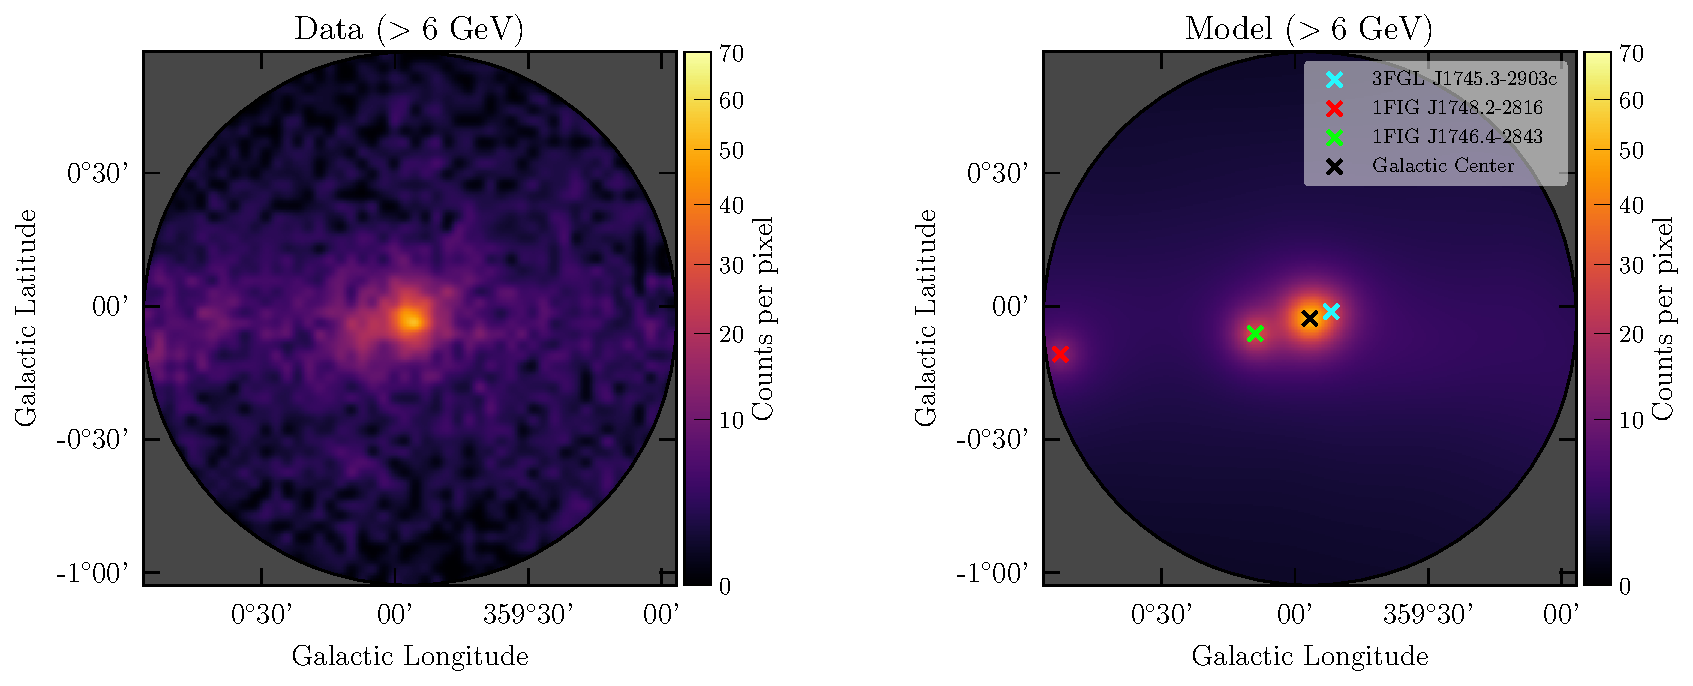
\includegraphics[width=0.9\columnwidth]{figures/dataModelComparison}
\noindent
\caption{ 
\label{fig:roi_residmap}
{\it Left panel:} Total photon counts in the ROI used in the analysis. The GC source is prominently seen near the center of the image, while the Galactic diffuse emission is responsible the majority of the photons outside the GC. {\it Right panel:} Model of the ROI after fitting with {{\tt gtlike}} (see Section \ref{sec:model_GC}), with the four point sources in the image labeled. In both maps, the pixel size is 0.04$^\circ$ and a Gaussian smoothing has been applied.
}
\end{center}
\end{figure}

\subsection{Modeling the Galactic Center}\label{sec:model_GC}

In order to search for a DM signal via the maximum-likelihood analysis described in Section \ref{sec:analysis}, we required a model of the ROI.
Our model was built from diffuse components and objects listed in the \textit{Fermi}-LAT Third Source Catalog (3FGL)~\cite{REF:2015.3FGL} and 1FIG~\cite{GC2016}. 

Once a model was defined, we compute its likelihood $\mathcal{L}(n,\theta)$ by:
\begin{equation}
\label{eq:likelihood}
\mathcal{L}(n, \theta) = \prod_{i=0}^{N}\frac{\mu_i^{n_i}}{n_i!}e^{-\mu_i}
\end{equation}
Where the index $i$ runs over the angular and energy bins, and $n$ is the actual data. 
We vary the model parameters $\theta$ until the likelihood is maximized; in practice we take the logarithm of the result. 
The likelihood computation and maximization was performed by the {\it Fermi} Science Tool \textup{gtlike}, which in turn used the MINUIT \cite{MINUIT} optimization routine.

\subsubsection{Diffuse Components and Extended Sources}\label{sec:diffuse}
Although a custom interstellar emission model (IEM) was successfully used to model the GC in previous works~\cite{GC2016} based on the Pass 7 data reconstruction, generating a similar custom IEM for the Pass 8 data used here was deemed to be outside the scope of this paper; the diffuse components used in this analysis were the standard Pass 8 models taken from the Fermi Science Support Center\footnote{The diffuse background models are available at: \url{http://fermi.gsfc.nasa.gov/ssc/data/access/lat/BackgroundModels.html} as {is\_P8R2\_SOURCE\_V6\_v06.txt} and {gll\_iem\_v06.fits}.}.
After fitting the data we found that the contribution of the isotropic component of our model was negligible when compared to the Galactic diffuse component; we decided not to include an isotropic component in the final model for this reason.

\subsubsection{Point Sources}
There are two point source catalogs that are relevant for our ROI: the 3FGL and 1FIG.
However, because our analysis covers a different time and energy range than either of the catalogs, it was not expected that either catalog would fit the data perfectly.
Instead, each catalog (along with the diffuse component from Section \ref{sec:diffuse} above) was used to fit the data separately, and sources that were insignificant above 10 GeV were excluded.
The three remaining sources were then used together to form our final model, which was found to yield better results than the results of each catalog individually.
For simplicity, we used a power law to describe the spectrum of all the sources in the model; none of the sources were fit significantly better by a curved spectrum over the energy range considered.

The GC is the most complicated region of the $\gamma$-ray sky, and as a result the point source associated with Sag A* is flagged in the 3FGL catalog as strongly dependent on the model of Galactic diffuse emission. 
However, a complete study of different diffuse emission models and their effects on the GC source properties was deemed outside the scope of this work, for which we needed only an empirical model against which we can test our DM hypothesis.

We found when fitting our data that the GC source was better fit by a narrow Gaussian distribution than a simple point source:
\begin{equation}
\rho (r) = \frac{1}{\sqrt{2\pi\sigma_r^2}}\exp{\frac{-r^2}{2\sigma_r^2}}
\end{equation}

with $\sigma_{r}=0.03^\circ$, and $r$ measured in degrees.
Although $\sigma$ is smaller than the {\it Fermi}-LAT PSF at 10 GeV, the extension was found to improve the residuals between the model and data, especially at the particular location of Sag A*- see Figure \ref{fig:residmapComparison}. 


\begin{figure}[ht] 
\begin{center}
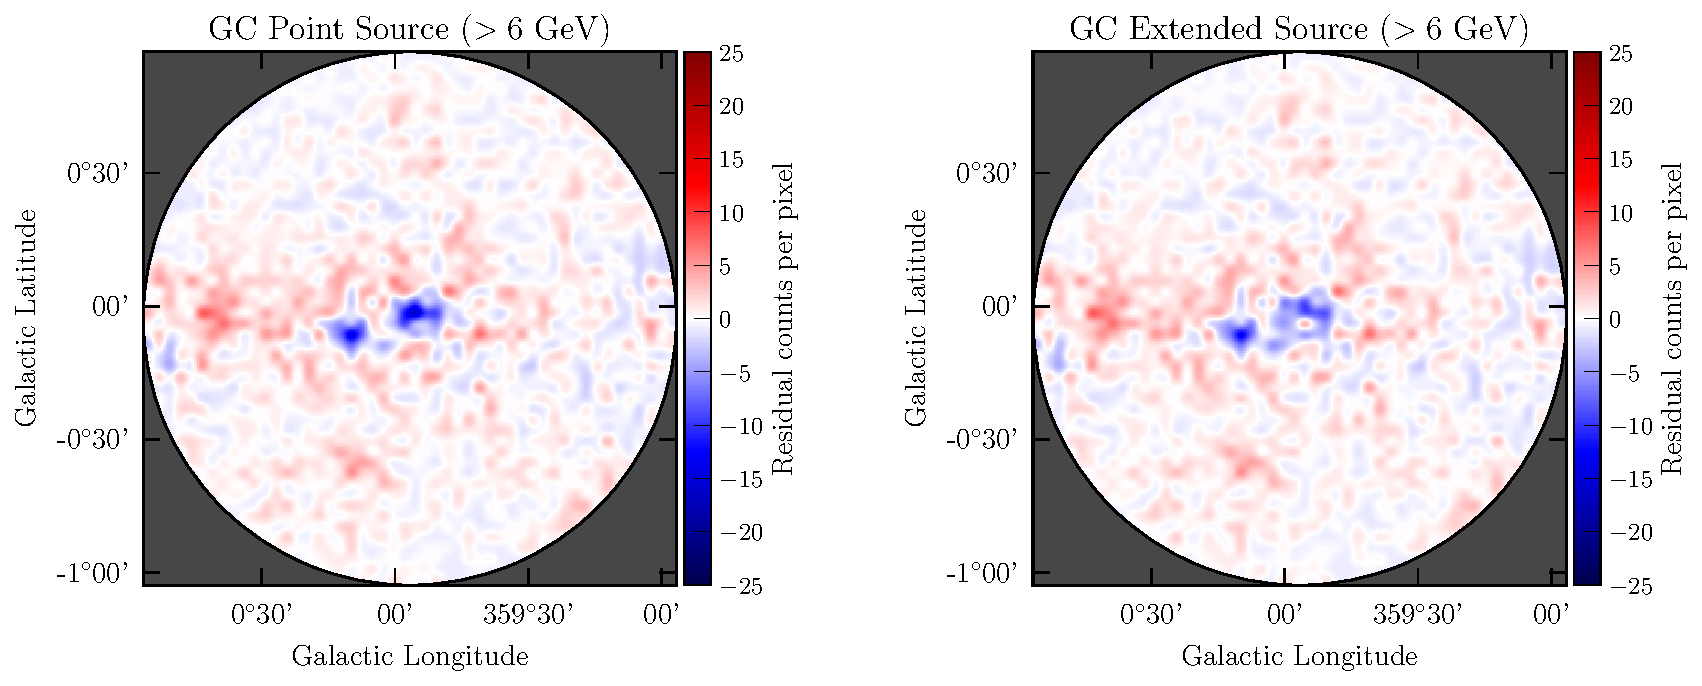
\includegraphics[width=0.9\columnwidth]{figures/residComparison.pdf}
\noindent
\caption{ 
\label{fig:residmapComparison}
{\it Left Panel}: The counts residuals for the best-fit model using a point source description of the Galactic Center source.
{\it Right Panel}: Residuals given a slightly extended source as described in the text, showing modest improvement at the location of Sag A. In both panels the angular pixelization and smoothing are the same as in Figure \ref{fig:roi_residmap}}
\end{center}
\end{figure}

A summary of the sources used in the model is shown in Table \ref{tab:model}, and the best-fit model (integrated over the energy range) is shown in the right panel of Figure \ref{fig:dataModelComparison}.

\begin{table}[ht]
\begin{tabularx}{\textwidth}{c @{\extracolsep{\fill}} ccccc}
\hline \hline
Source Description & Spectral Model & $N_{\gamma}$ & Spatial Model & RA & DEC\\ \hline
Galactic diffuse emission & PowerLaw & 4397 & MapCube & - & - \\ 
GC & PowerLaw & 1337 & Gaussian distribution, $\sigma = 0.03^{\circ}$ & 266.42 & -29.01 \\
1FIG J1746.4-2843 & PowerLaw & 536 & Point Source & 266.59 & -28.86 \\
1FIG J1748.2-2816 & PowerLaw & 176 & Point Source & 267.10 & -28.28 \\
3FGL J1745.3-2903c & PowerLaw & 169 & Point Source & 266.34 & -29.06 \\
\hline
\end{tabularx}
\caption{ \label{tab:model} List of sources used in modeling the ROI. }
\end{table}

As a check of our systematic uncertainty, we also performed the following analysis using a separate dataset covering 4 years of data with Pass 7 data reconstruction.
The model of the ROI contained the same point sources as presented here, however the diffuse models were the custom Pass 7 models from the work in \citep{GC2016}. 
The resulting flux upper limits were found to be consistent with the main analysis presented below- for simplicity we present only the standard analysis with Pass 8 data reconstruction.

%In the most conservative possible model, one could remove the GC source and consider all the flux from the Galactic Center as originating from DM annihilation.
%Although we do not regard this model as physically realistic, we analyzed this case separately and found the resulting upper limits on the annihilation flux to be about a factor of $10^2$ greater across the energy range considered.

\section{ANALYSIS}\label{sec:analysis}


\subsection{Fitting Method}\label{sec:fitting}
As discussed in Section \ref{sec:dm}, the phenomenology of our reference model p-wave DM signal is that of a point source located at the location of Sag A*, with an energy spectrum that is flat between two endpoints (a `box' shape).
For this analysis, we considered two representative versions of the box: the `wide' box has a value of $\zeta = 0.44$, while the `narrow' box has a value of $\zeta = 0.9999$.
Implications from the two types of searches for mass splittings in intermediate cases are discussed in Section \ref{sec:conclusion}.

We searched for $\gamma$-ray boxes which had an upper-edge energy equal to the boundaries of the energy bins between 10 and 658 GeV in our data selection, corresponding to 42 different DM hypotheses.
In order to prevent edge effects from impacting the results, boxes with upper edges outside of this range were not considered. 
An example DM signal (integrated over the ROI), along with the background, is shown in the left panel of Figure \ref{fig:artificial_box}. 

The significance of each DM hypothesis was evaluated using the test statistic (TS) defined as: 
\begin{equation}
\mathrm{TS}=2~\mathrm{ln}\frac{\mathcal{L}(\mu, \theta | \mathcal{D})}{\mathcal{L}_{\mathrm{null}}(\theta | \mathcal{D})} \label{eq:ts}
\end{equation}
Where $\mu$ is the signal strength, $\theta$ is the array of parameters describing the DM hypothesis (in this case, the energy and width of the $\gamma$-ray box, and $\mathcal{D}$ represents the binned data. $\mathcal{L}_{\mathrm{null}}$ is the value of the likelihood in the absence of any signal.
The likelihood values $\mathcal{L}$ are computed from Equation \ref{eq:likelihood}.

The TS value was then used to calculate a level of significance $Z$ via:
\begin{equation}
Z = \Phi ^{-1} \left( 1-\int_\mathrm{TS}^\infty \chi^2(x,k)dx\right)
\end{equation}
Where $\Phi ^{-1}$ is the inverse quantile function; the integral in this expression is the $p$-value.
Simulations (described below) confirmed that the TS values were distributed following a $\chi^2$ distribution with 1 degree of freedom (the total flux contained in the `box' signal)- see the left panel of Figure \ref{fig:correlations}. As the counts per bin decreases, the $\chi^{2}$ distribution moderately over-predicts the number of high TS trials observed in simulated data. 

The procedure for finding the TS of a given DM hypothesis and upper limit on the total flux of a $\gamma$-ray box with an upper edge at a particular bin energy was as follows:
\begin{enumerate}\label{sec:procedure}
\item \label{step:fit} The parameters of the model described in Section \ref{sec:model_GC} allowed to vary to maximize the likelihood function $\mathcal{L}$, giving the null likelihood.
This step was performed once for each set of 42 DM hypotheses that corresponded to the dataset under investigation (either the actual data or the Poisson fluctuations described below). 
\item The expected spectrum of the DM signal is calculated by convolving a ideal box spectrum with a Gaussian distribution representing with the \Fermi-LAT energy resolution, which is between 5\% and 10\% in the energy range considered. 
\item A point-source with the convolved DM spectrum is added to the model at the location of Sag A*, with a single overall normalization parameter $N$.
\item All parameters in the model except for the normalization of the central GC source are fixed.
A study of the correlation coefficients (see Section \ref{sec:correlations}) showed that the signal was modestly correlated with this source, but had negligible correlation with other parameters in the model.
Fixing the other parameters has the benefit of decreasing the computation time and preventing numerical instabilities when fitting a system with a large number of degrees of freedom.
\item The normalization $N$ of the DM source is increased from a value of 0 until the TS exceeds 2.71, which corresponds to a 95\% confidence upper limit on $N$, or a $Z$ value of approximately 2. The value of $N$ for which $\mathcal{L}$ is maximized and the corresponding TS are also stored in order to evaluate the significance of the best-fit DM hypothesis.
\end{enumerate}



\subsection{Correlations Between Background and Signal Components}\label{sec:correlations}

In order to understand the relationship between a potential signal and the background sources, we calculated the correlation coefficients between the signal source and the GC source.
As expected, both $\zeta=0.9999$ and $\zeta=0.44$ hypotheses are negatively correlated with the normalization of the GC background source.
We found that the signal became less correlated as the right edge of the box increases in energy, since the likelihood fit is strongly driven by the higher statistics at low energy.
We also found that the $\zeta=0.44$ hypothesis had a stronger correlation to the background when compared to the  $\zeta=0.9999$ case, which is expected because the $\zeta=0.44$ signal contributes over a broader energy range. 

A plot of the correlation coefficients in both cases as a function of the energy of the right edge of the box is shown in the right panel of Figure \ref{fig:correlations} below.
Because the GC source has a power-law spectral shape, its prefactor and index were found to be almost perfectly anticorrelated (correlation coefficient $<$-0.95), and therefore the correlation coefficient between the signal and GC index was nearly identical to that between the signal and GC prefactor.
We found that the correlation coefficients of the signal to the parameters of other sources in the model were negligible.

\begin{figure}[ht] 
\begin{center}
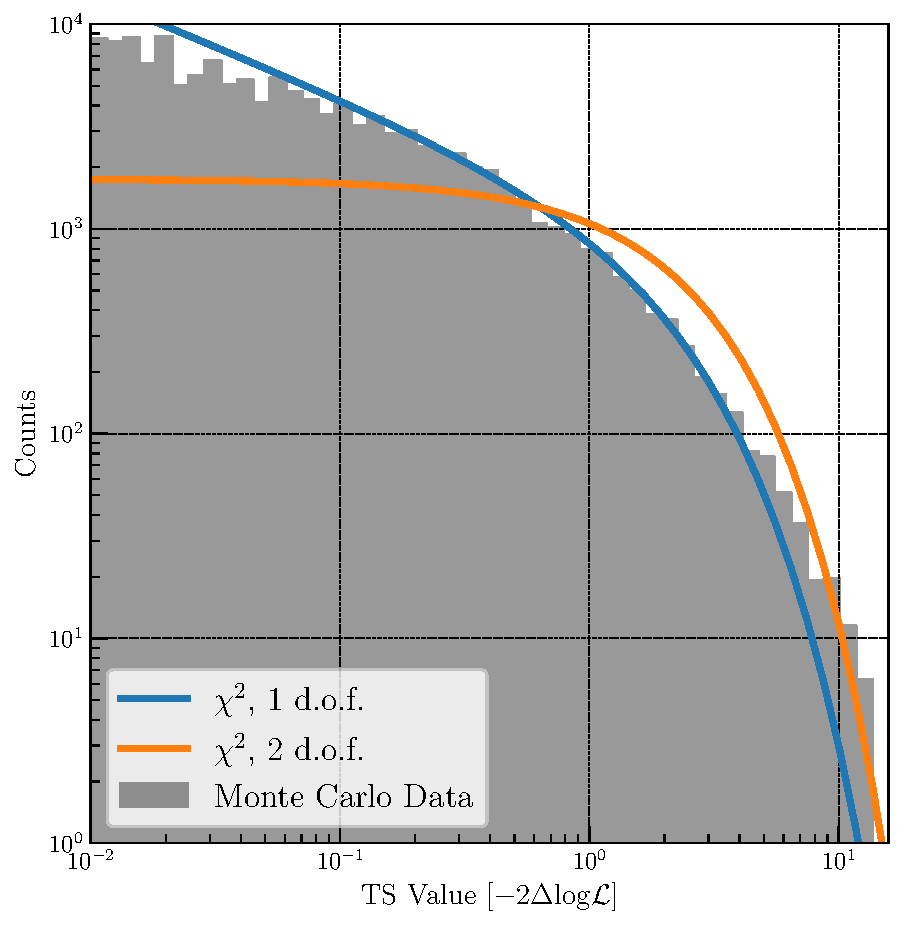
\includegraphics[width=0.45\columnwidth]{figures/ts_hist.pdf}
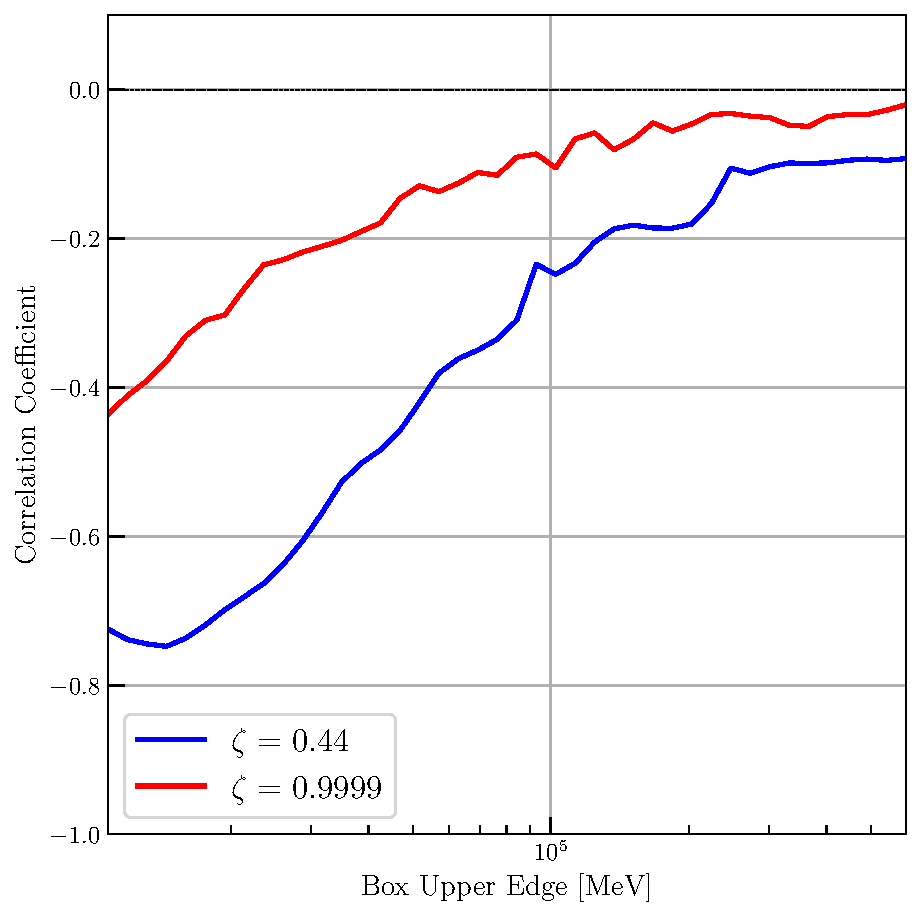
\includegraphics[width=0.45\columnwidth]{figures/correlation_coefficients.pdf}
\noindent
\caption{ 
\label{fig:correlations}
{\it Left Panel}: Histogram of TS values for all DM signal hypotheses from the Monte Carlo study for a $\zeta=0.44$ signal. The shape of the TS distribution is best-fit by a $\chi^2$ distribution with only one degree of freedom, although the $\chi^2$ distribution slightly underpredicts the true distribution at high TS. At the critical value of 2.71, the shape of the distribution is particularly well-described by the $\chi^2$ distribution. 
{\it Right Panel}: Correlation coefficients between the total flux of the DM signal hypotheses and the normalization $N$ of the GC source (modeled here as a power law, i.e. $\frac{dN}{dE} = Ne^{-\alpha E}$.
We evaluate the correlation as a function of the upper edge of the DM signal box, and find that the correlation is negligible for high-energy boxes but is becomes significant at lower energies because of the increased statistics in the data.
Because the two sources are spatially coincident, the sources are expected to be anticorrelated.
}
\end{center}
\end{figure}

\subsection{Monte Carlo Simulations\label{sec:MCMethods}}
We performed a Monte Carlo study in order to understand the impact that statistical fluctuations have on the analysis. 
Each instance of the Monte Carlo began by generating Poissonian fluctuations about the best-fit model of the data.
We then used the Poisson data as the input to the protocol defined in Section \ref{sec:fitting}, and stored both the upper limit and TS values for each DM hypothesis.
Because Step \ref{step:fit} above fits the parameters of the background model, this technique probes the effects of statistical uncertainty on both the signal and the background.
We performed O($10^3$) simulations, and used the upper limit curves from each instance to generate 68\% and 95\% containment bands in the cases of $\zeta = 0.44$ and $\zeta = 0.9999$.
The upper limits from the data and the containment bands from the Monte Carlo study are displayed in Figure \ref{fig:brazil_lines}.

\subsection{Reconstruction of Injected Signal\label{sec:injected}}
To confirm that the upper limit calculation was sensitive to the presence of a DM signal, and to understand how a signal would appear in our analysis, we injected a DM signal into the data and repeated the analysis procedure from Section \ref{sec:procedure}.
The injected DM signal for this test was defined to have $\zeta = 0.44$ and a total flux of $3.0*10^{-10} $ph cm$^{-2} $s$^{-1}$, with an upper energy endpoint of 100 GeV.
At 100 GeV, the ratio of the injected signal flux to the total flux in the ROI was about 30\%.
We performed the same Monte Carlo study on the injected-signal dataset to produce containment bands for the limit.

The results of the analysis are in good agreement with the known injected signal.
The best-fit DM hypothesis was found to have an upper edge energy of 102 GeV, and the reconstructed flux of the signal was $3.7*10^{-10}$ ph cm$^{-2} $s$^{-1}$; moreover, the signal was highly significant (TS=167).
The upper limit curve was found to contain a prominent bump near 100 GeV which noticeably exceeded the 68\% and 95\% containment bands from the Monte Carlo study, as seen in Figure \ref{fig:artificial_box}.
%The upper limit at 100 GeV was $4.5*10^{-10}$ ph cm$^{-2} $s$^{-1}$.  
We concluded that the analysis procedure defined in Section \ref{sec:fitting} is sensitive to the presence of a realistic DM signal, and can accurately reconstruct its parameters.
The best-fit box is shown in the left panel of Figure \ref{fig:artificial_box}.


\begin{figure}[ht]
\begin{center}
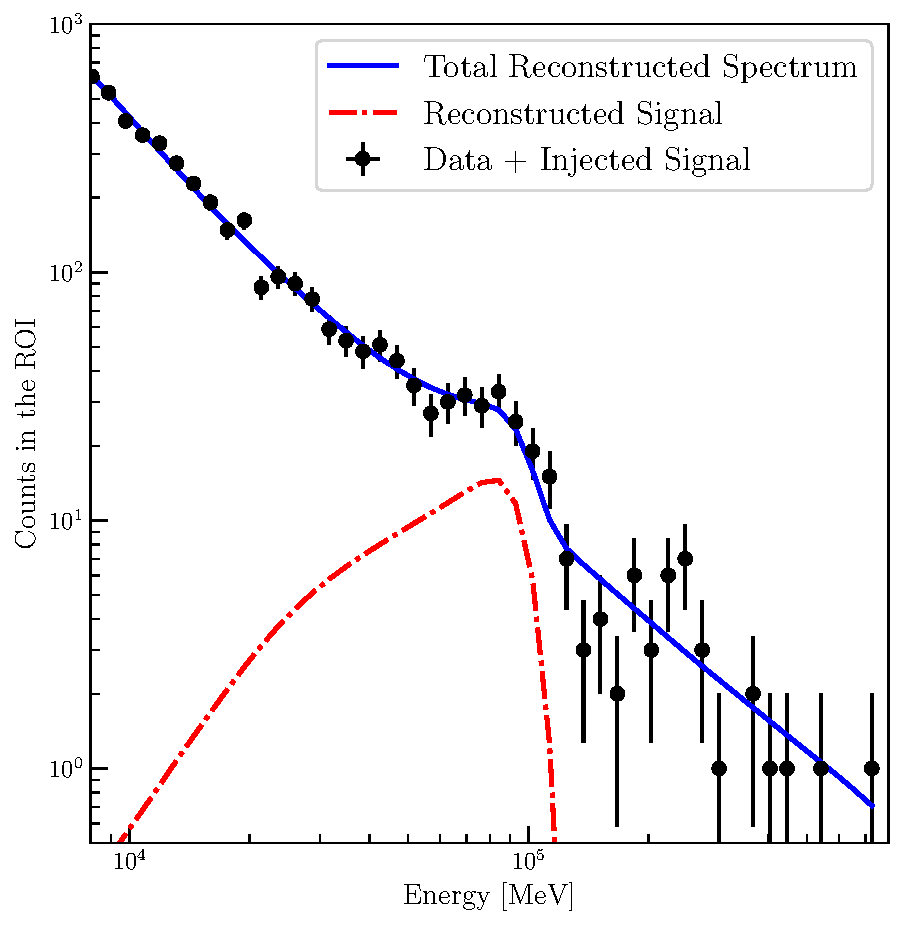
\includegraphics[width=0.45\columnwidth]{./figures/good_box_fit.pdf}
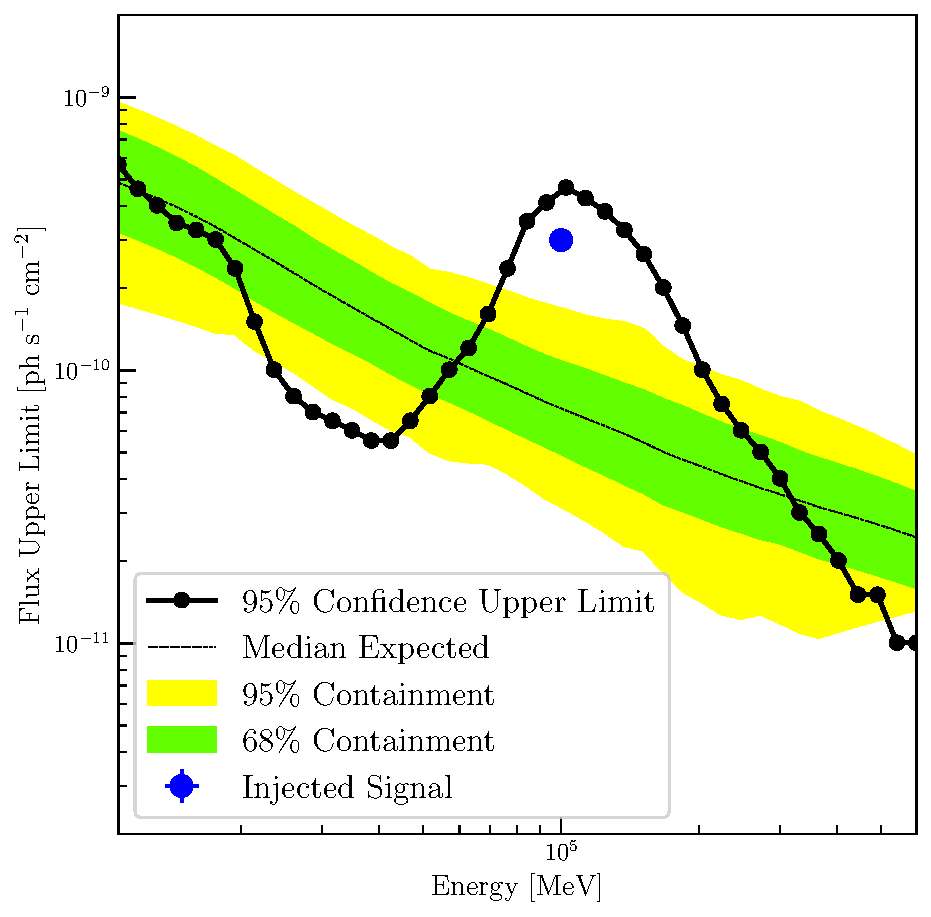
\includegraphics[width=0.45\columnwidth]{./figures/brazil_artificial_box.pdf}
\noindent
\caption{
\label{fig:artificial_box}
{\it Left Panel}: Energy spectrum of the data + injected signal. The 'box' DM signal appears as a prominent bump near its upper endpoint. 
{\it Right Panel}: The DM signal upper limit (in black) in the presence of an injected box with upper endpoint 100 GeV and total flux $3*10^{-11} $ ph cm$^{-2} $s$^{-1}$. The blue dot shows the position of the injected signal.
The 68\% and 95\% containment bands are constructed from performing the analysis on Poisson-fluctuated datasets about the best-fit background model. 
Our injected DM signal is not excluded by the analysis. 
}
\end{center}
\end{figure}


\section{Results}\label{sec:results}

No significant signal from a p-wave DM signal was seen in either the case of the wide or narrow box.
The flux upper limits are shown in Figure~\ref{fig:brazil_narrow_box} for both the wide box (left panel) and the narrow box (right panel) scenarios. 
The strongest signal came in the case of $\zeta = 0.9999$ at energy 247 GeV; the TS of this DM hypothesis was 4.0, corresponding to a local significance of 1.7$\sigma$ with one degree of freedom.
In the case of $\zeta = 0.44$, the strongest signal came from a box with an upper-edge energy of 17 GeV; the TS of the signal was 3.5 for a significance of 1.5$\sigma$.
These do not take into account trials factors, so their global significance is reduced further.

\begin{figure}[ht] 
\begin{center}
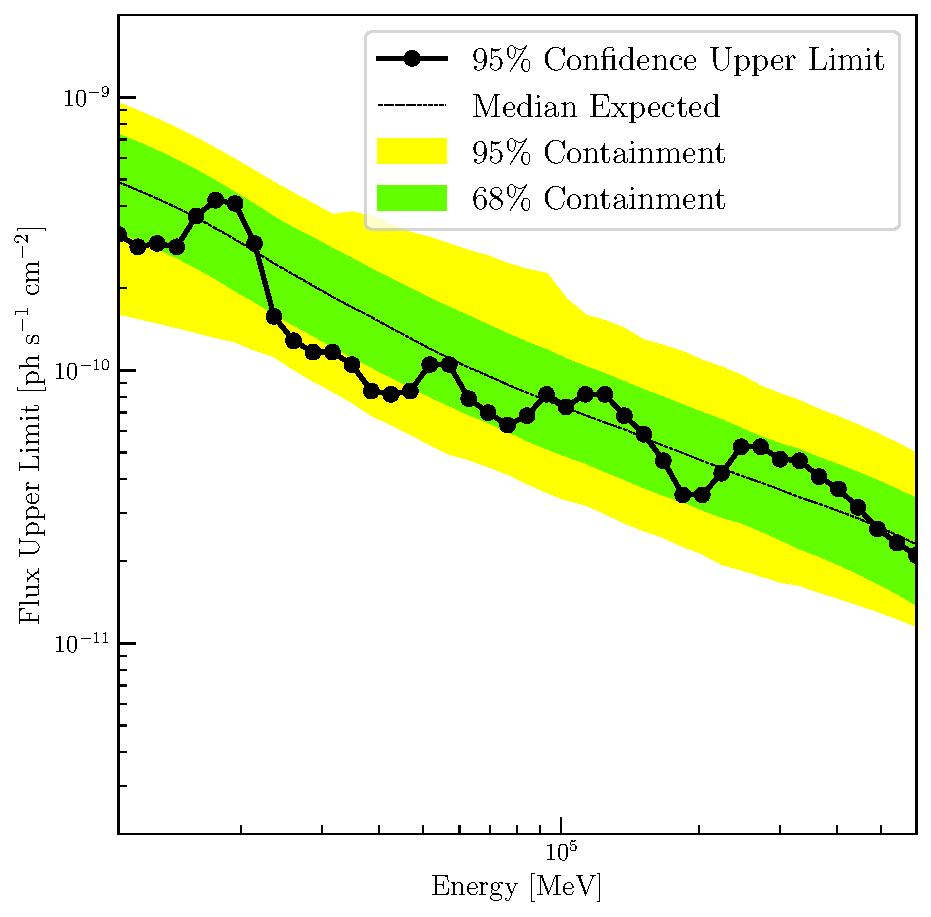
\includegraphics[width=0.45\columnwidth]{figures/brazil_wide_box.pdf}
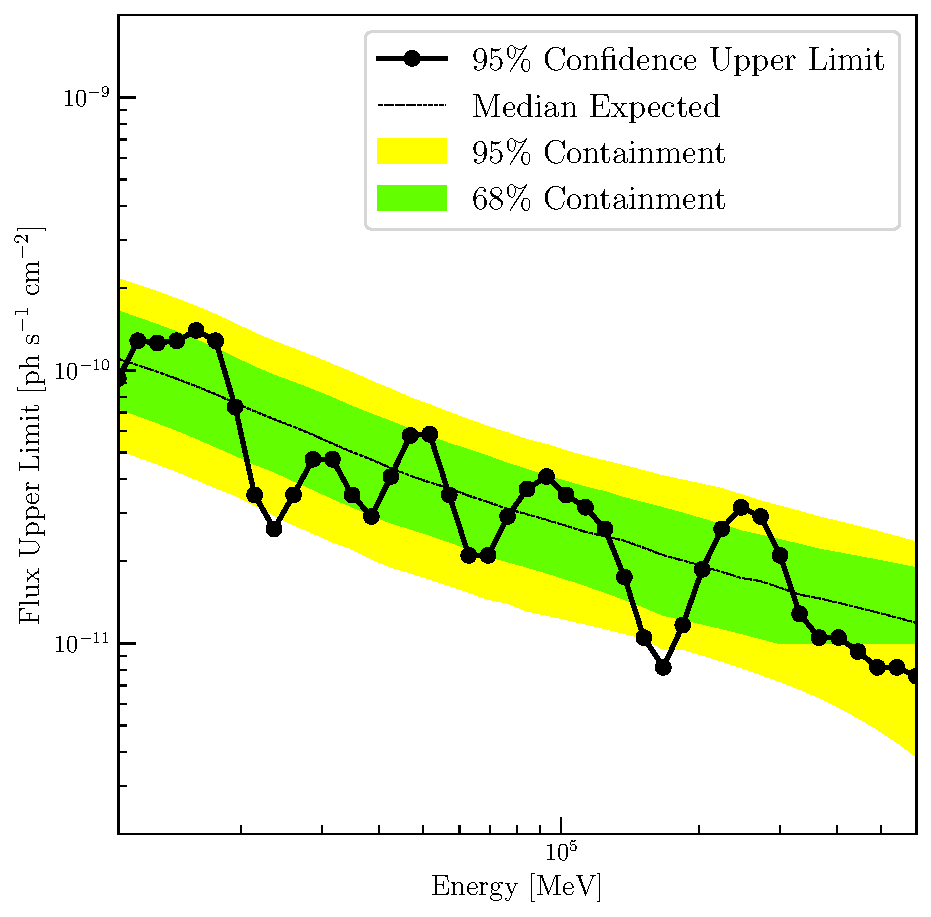
\includegraphics[width=0.45\columnwidth]{figures/brazil_narrow_box.pdf}
\noindent
\caption{ 
\label{fig:brazil_lines}
95\% confidence flux upper limit on a $\gamma$-ray box point source at the GC. In the left figure, the box extends from 0 GeV to the energy indicated (wide box). On the right, the width of the box is 1 GeV (narrow box). The 68\% and 95\% containment bands come from a Monte Carlo simulation of the data described in Section \ref{sec:MCMethods}. \label{fig:brazil_narrow_box}
}
\end{center}
\end{figure}

%\begin{figure}[ht] 
%\begin{center}
%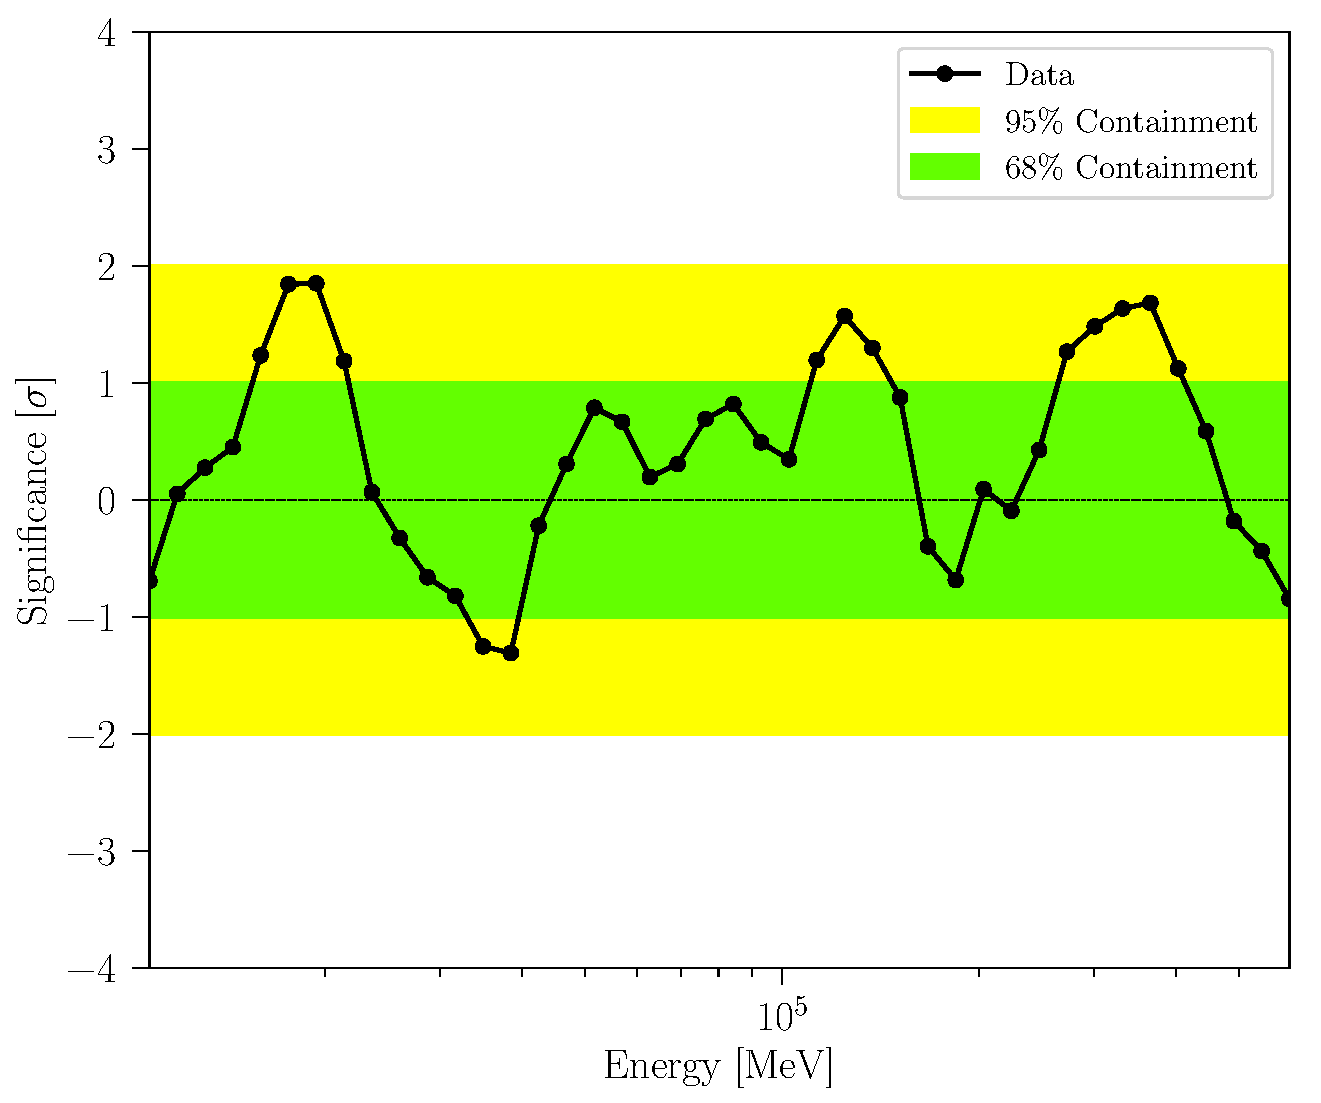
\includegraphics[width=0.45\columnwidth]{figures/significance_wide_box.pdf}
%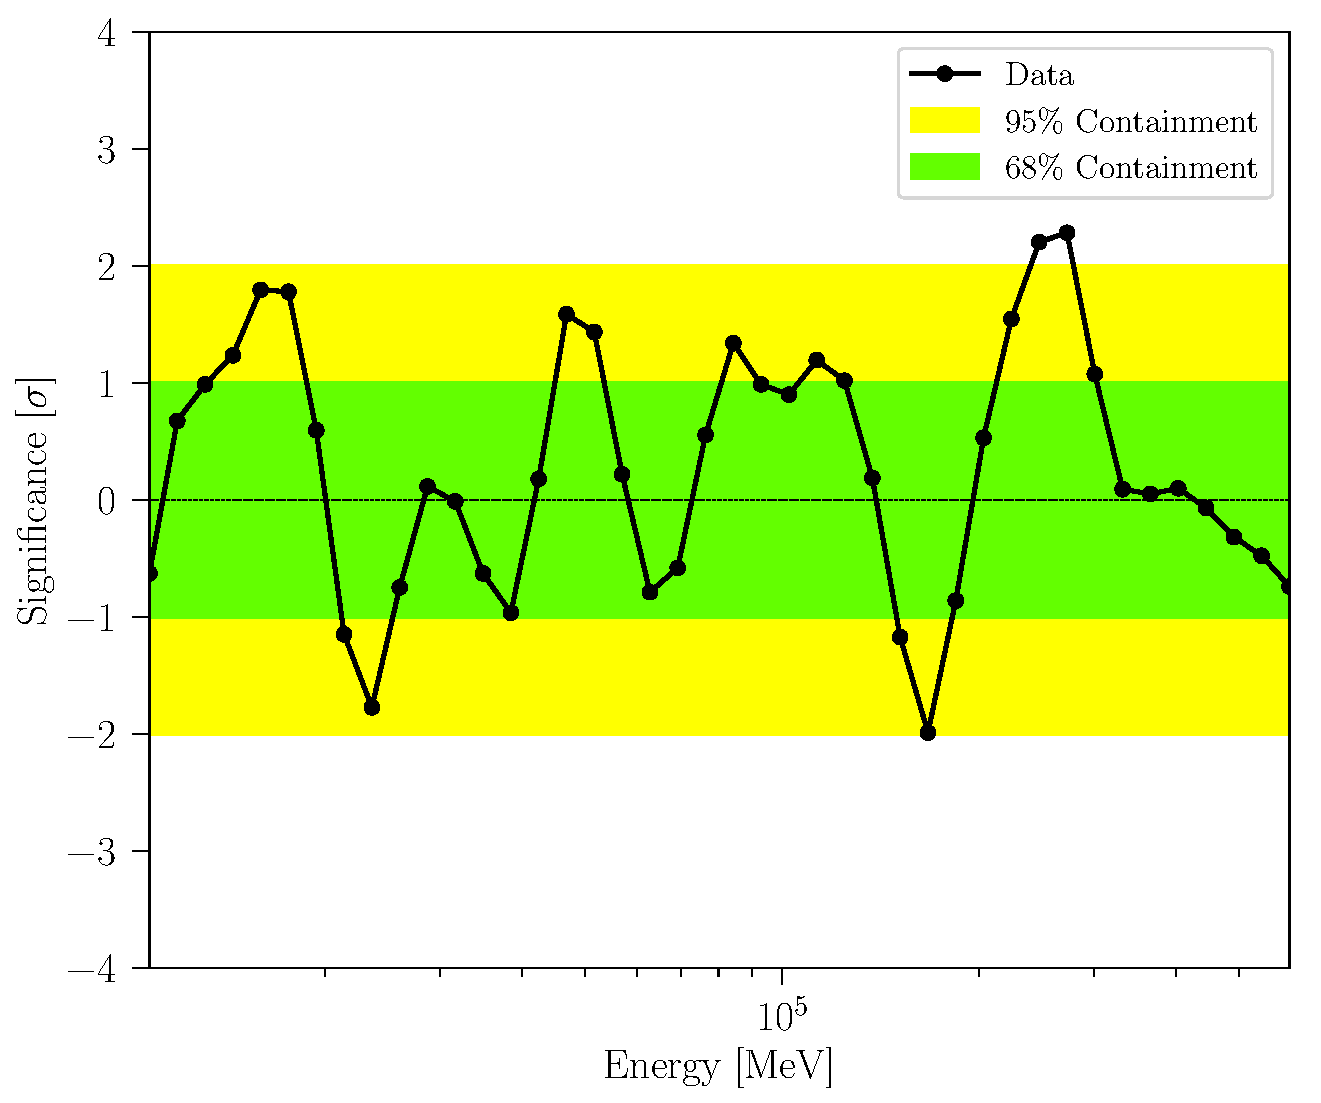
\includegraphics[width=0.45\columnwidth]{figures/significance_narrow_box.pdf}
%\noindent
%\caption{ 
%\label{fig:significances}
%The significance curves for the wide box case on the left, and the narrow box case on the right. In both cases the most significant bump occurs at around 16 GeV; the bump has a local significance of 2.3$\sigma$ in the wide-box case and a local significance of 2.9$\sigma$ in the narrow-box case. The global significances are 0.3$\sigma$ and 1.4$\sigma$, respectively.
%}
%\end{center}
%\end{figure}

The predicted flux from $p$-wave DM annihilation depends on the DM mass $m_{DM}$ as well as on the power laws of the DM halo ($\gamma_c$) and spike ($\gamma_{sp}$) in our fiducial model.  In Figure~\ref{fig:final_interp} we fix the DM mass, and show how the upper limits on narrow and wide boxes constrain the allowed DM distribution in the GC.  We can observe in particular that adiabatic spikes are excluded for even very shallow cusps $\gamma_c = 0.8$.  In this parameter space, DM models yielding narrow boxes are less constrained than DM models yielding wide boxes, despite the stronger flux limits; this occurs because the limited phase space available for the narrow box annihilation process further suppresses the annihilation.




\begin{figure}[ht] 
\begin{center}
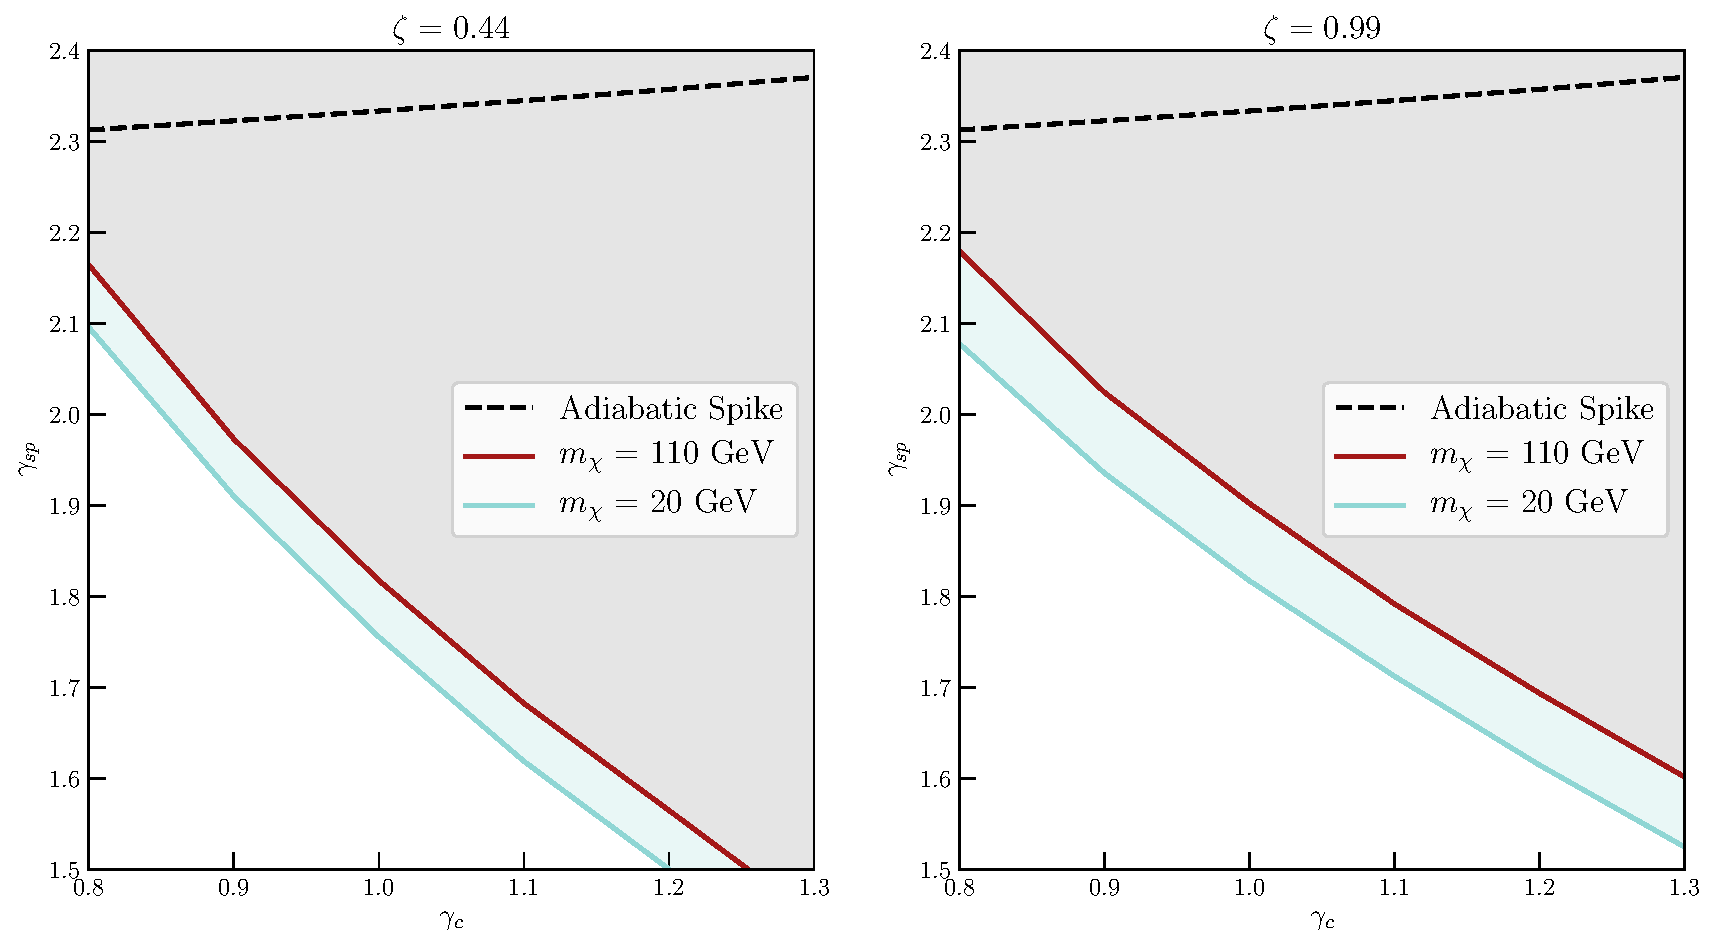
\includegraphics[width=0.9\columnwidth]{figures/final_interpretation.pdf}
\noindent
\caption{ 
\label{fig:final_interp}
DM distributions in the GC compatible with thermal relic $p$-wave DM in the hidden sector axion portal model, shown for two representative choices of DM mass $m_\chi = 20$ GeV, 110 GeV for narrow boxes (left, $\zeta=0.99$) and wide boxes (right, $\zeta = 0.44$).
}
\end{center}
\end{figure}

In Figure~\ref{fig:near-final} we consider fixed sample choices of $\gamma_c$ and $\gamma_{sp}$ and show the resulting limits on our reference hidden sector axion portal $p$-wave DM model as a function of DM mass.  For clarity we plot the ratio of the excluded cross-section $\langle\sigma v\rangle$ to the value of the cross-section that yields the correct relic abundance, $\langle\sigma v\rangle_{\mathrm{thermal}}$.  We comment that exclusions for the narrow box scenario in this reference model should not be considered literally at high masses as the model becomes non-perturbative above $m_\chi\sim 300$ GeV.  The need for such large couplings arises to compensate for the phase space suppression that follows when $m_\chi\approx m_\phi$, and no such issue arises in the wide box scenario.


\begin{figure}[ht] 
\begin{center}
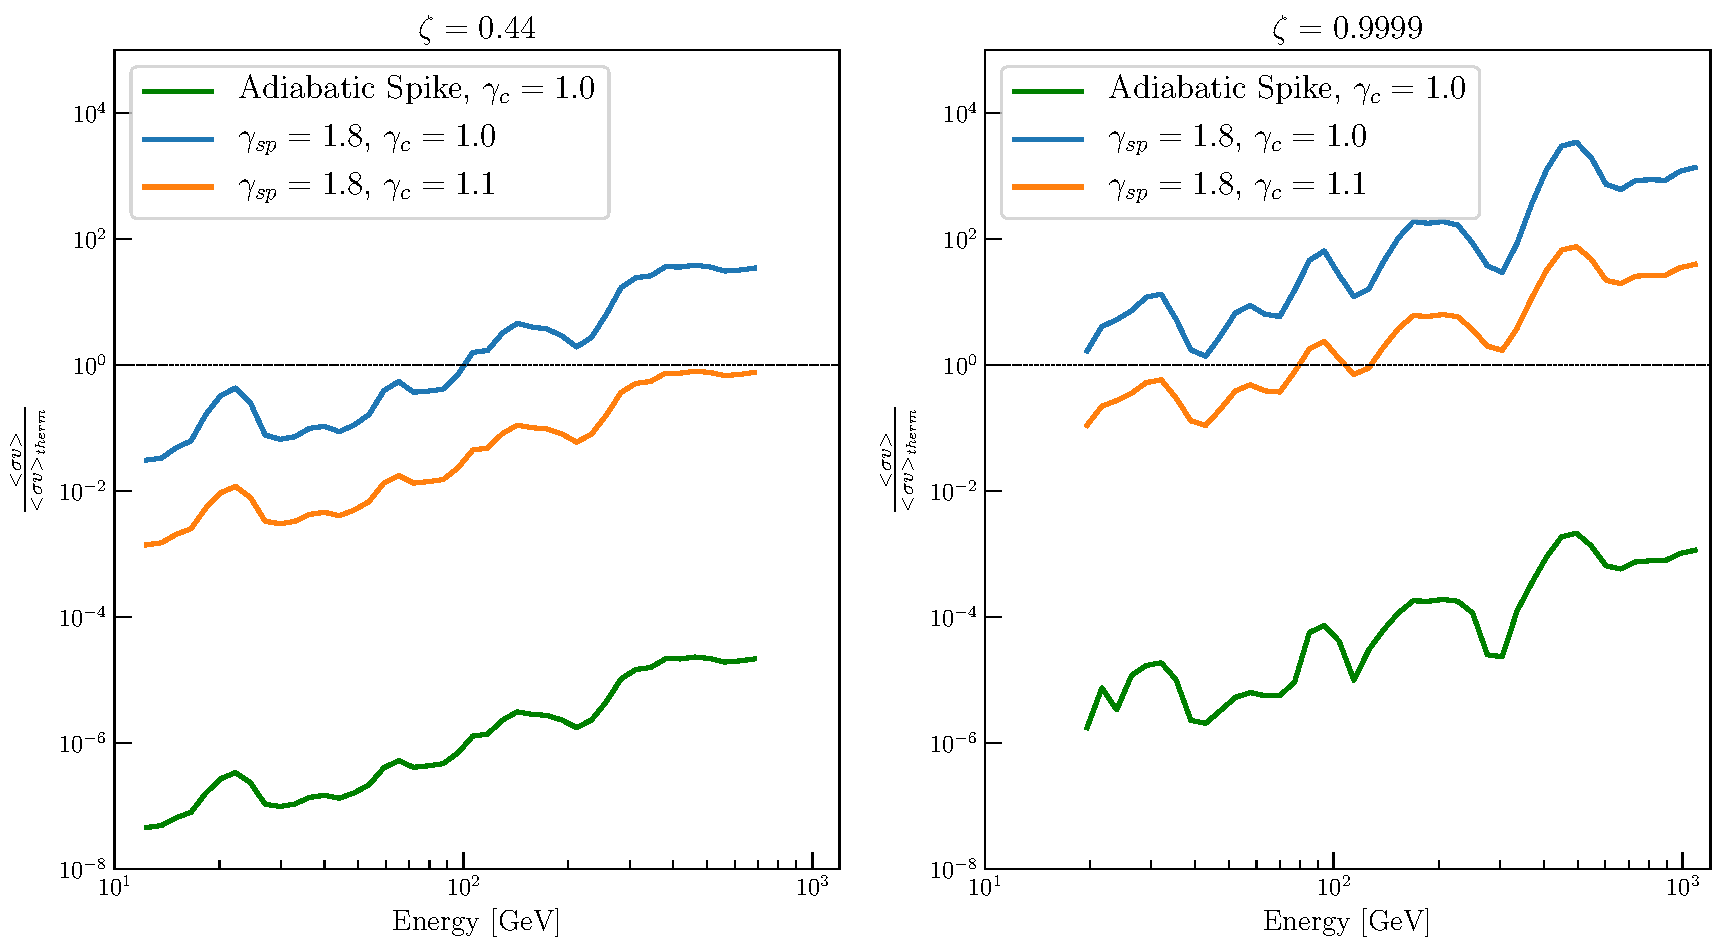
\includegraphics[width=0.9\columnwidth]{figures/final_fixed_astro.pdf}
\noindent
\caption{ 
\label{fig:near-final}
Limits on DM annihilation cross-section as a function of DM mass for fixed values of $\gamma_c$, $\gamma_{sp}$.   For clarity we plot the velocity-independent ratio of the excluded cross-section to the value that yields the correct relic abundance.  From top to bottom, the three curves correspond to  $\gamma_c = 1.1, \gamma_{sp}=1.8$ (orange);  $\gamma_c = 1.0, \gamma_{sp}=1.8$ (blue); and $\gamma_c = 1, \gamma_{sp}=2.33$ (adiabatic spike, green).
}
\end{center}
\end{figure}

% %%%%%%%%%%%%%%%%%%%%%%%%%%%%%%%%%%%%%%%%%%%%%%%%%%%%%%%%%
% bibliography

% 2010june01 sol katzman:
% if \nocite is specified, all entries in the bib file are included,
% probably not what you want, so comment out the \nocite and only get the cited references.
%\nocite{*}

% 2010june01 sol katzman:
% this makes the bibliography single spaced, with double spacing between entries
\def\baselinestretch{1.0}\large\normalsize

\bibliographystyle{plain}
\bibliography{uctest}

\end{document}
